% Options for packages loaded elsewhere
% Options for packages loaded elsewhere
\PassOptionsToPackage{unicode}{hyperref}
\PassOptionsToPackage{hyphens}{url}
\PassOptionsToPackage{dvipsnames,svgnames,x11names}{xcolor}
%
\documentclass[
  letterpaper,
  DIV=11,
  numbers=noendperiod]{scrreprt}
\usepackage{xcolor}
\usepackage{amsmath,amssymb}
\setcounter{secnumdepth}{5}
\usepackage{iftex}
\ifPDFTeX
  \usepackage[T1]{fontenc}
  \usepackage[utf8]{inputenc}
  \usepackage{textcomp} % provide euro and other symbols
\else % if luatex or xetex
  \usepackage{unicode-math} % this also loads fontspec
  \defaultfontfeatures{Scale=MatchLowercase}
  \defaultfontfeatures[\rmfamily]{Ligatures=TeX,Scale=1}
\fi
\usepackage{lmodern}
\ifPDFTeX\else
  % xetex/luatex font selection
\fi
% Use upquote if available, for straight quotes in verbatim environments
\IfFileExists{upquote.sty}{\usepackage{upquote}}{}
\IfFileExists{microtype.sty}{% use microtype if available
  \usepackage[]{microtype}
  \UseMicrotypeSet[protrusion]{basicmath} % disable protrusion for tt fonts
}{}
\makeatletter
\@ifundefined{KOMAClassName}{% if non-KOMA class
  \IfFileExists{parskip.sty}{%
    \usepackage{parskip}
  }{% else
    \setlength{\parindent}{0pt}
    \setlength{\parskip}{6pt plus 2pt minus 1pt}}
}{% if KOMA class
  \KOMAoptions{parskip=half}}
\makeatother
% Make \paragraph and \subparagraph free-standing
\makeatletter
\ifx\paragraph\undefined\else
  \let\oldparagraph\paragraph
  \renewcommand{\paragraph}{
    \@ifstar
      \xxxParagraphStar
      \xxxParagraphNoStar
  }
  \newcommand{\xxxParagraphStar}[1]{\oldparagraph*{#1}\mbox{}}
  \newcommand{\xxxParagraphNoStar}[1]{\oldparagraph{#1}\mbox{}}
\fi
\ifx\subparagraph\undefined\else
  \let\oldsubparagraph\subparagraph
  \renewcommand{\subparagraph}{
    \@ifstar
      \xxxSubParagraphStar
      \xxxSubParagraphNoStar
  }
  \newcommand{\xxxSubParagraphStar}[1]{\oldsubparagraph*{#1}\mbox{}}
  \newcommand{\xxxSubParagraphNoStar}[1]{\oldsubparagraph{#1}\mbox{}}
\fi
\makeatother

\usepackage{color}
\usepackage{fancyvrb}
\newcommand{\VerbBar}{|}
\newcommand{\VERB}{\Verb[commandchars=\\\{\}]}
\DefineVerbatimEnvironment{Highlighting}{Verbatim}{commandchars=\\\{\}}
% Add ',fontsize=\small' for more characters per line
\usepackage{framed}
\definecolor{shadecolor}{RGB}{241,243,245}
\newenvironment{Shaded}{\begin{snugshade}}{\end{snugshade}}
\newcommand{\AlertTok}[1]{\textcolor[rgb]{0.68,0.00,0.00}{#1}}
\newcommand{\AnnotationTok}[1]{\textcolor[rgb]{0.37,0.37,0.37}{#1}}
\newcommand{\AttributeTok}[1]{\textcolor[rgb]{0.40,0.45,0.13}{#1}}
\newcommand{\BaseNTok}[1]{\textcolor[rgb]{0.68,0.00,0.00}{#1}}
\newcommand{\BuiltInTok}[1]{\textcolor[rgb]{0.00,0.23,0.31}{#1}}
\newcommand{\CharTok}[1]{\textcolor[rgb]{0.13,0.47,0.30}{#1}}
\newcommand{\CommentTok}[1]{\textcolor[rgb]{0.37,0.37,0.37}{#1}}
\newcommand{\CommentVarTok}[1]{\textcolor[rgb]{0.37,0.37,0.37}{\textit{#1}}}
\newcommand{\ConstantTok}[1]{\textcolor[rgb]{0.56,0.35,0.01}{#1}}
\newcommand{\ControlFlowTok}[1]{\textcolor[rgb]{0.00,0.23,0.31}{\textbf{#1}}}
\newcommand{\DataTypeTok}[1]{\textcolor[rgb]{0.68,0.00,0.00}{#1}}
\newcommand{\DecValTok}[1]{\textcolor[rgb]{0.68,0.00,0.00}{#1}}
\newcommand{\DocumentationTok}[1]{\textcolor[rgb]{0.37,0.37,0.37}{\textit{#1}}}
\newcommand{\ErrorTok}[1]{\textcolor[rgb]{0.68,0.00,0.00}{#1}}
\newcommand{\ExtensionTok}[1]{\textcolor[rgb]{0.00,0.23,0.31}{#1}}
\newcommand{\FloatTok}[1]{\textcolor[rgb]{0.68,0.00,0.00}{#1}}
\newcommand{\FunctionTok}[1]{\textcolor[rgb]{0.28,0.35,0.67}{#1}}
\newcommand{\ImportTok}[1]{\textcolor[rgb]{0.00,0.46,0.62}{#1}}
\newcommand{\InformationTok}[1]{\textcolor[rgb]{0.37,0.37,0.37}{#1}}
\newcommand{\KeywordTok}[1]{\textcolor[rgb]{0.00,0.23,0.31}{\textbf{#1}}}
\newcommand{\NormalTok}[1]{\textcolor[rgb]{0.00,0.23,0.31}{#1}}
\newcommand{\OperatorTok}[1]{\textcolor[rgb]{0.37,0.37,0.37}{#1}}
\newcommand{\OtherTok}[1]{\textcolor[rgb]{0.00,0.23,0.31}{#1}}
\newcommand{\PreprocessorTok}[1]{\textcolor[rgb]{0.68,0.00,0.00}{#1}}
\newcommand{\RegionMarkerTok}[1]{\textcolor[rgb]{0.00,0.23,0.31}{#1}}
\newcommand{\SpecialCharTok}[1]{\textcolor[rgb]{0.37,0.37,0.37}{#1}}
\newcommand{\SpecialStringTok}[1]{\textcolor[rgb]{0.13,0.47,0.30}{#1}}
\newcommand{\StringTok}[1]{\textcolor[rgb]{0.13,0.47,0.30}{#1}}
\newcommand{\VariableTok}[1]{\textcolor[rgb]{0.07,0.07,0.07}{#1}}
\newcommand{\VerbatimStringTok}[1]{\textcolor[rgb]{0.13,0.47,0.30}{#1}}
\newcommand{\WarningTok}[1]{\textcolor[rgb]{0.37,0.37,0.37}{\textit{#1}}}

\usepackage{longtable,booktabs,array}
\usepackage{calc} % for calculating minipage widths
% Correct order of tables after \paragraph or \subparagraph
\usepackage{etoolbox}
\makeatletter
\patchcmd\longtable{\par}{\if@noskipsec\mbox{}\fi\par}{}{}
\makeatother
% Allow footnotes in longtable head/foot
\IfFileExists{footnotehyper.sty}{\usepackage{footnotehyper}}{\usepackage{footnote}}
\makesavenoteenv{longtable}
\usepackage{graphicx}
\makeatletter
\newsavebox\pandoc@box
\newcommand*\pandocbounded[1]{% scales image to fit in text height/width
  \sbox\pandoc@box{#1}%
  \Gscale@div\@tempa{\textheight}{\dimexpr\ht\pandoc@box+\dp\pandoc@box\relax}%
  \Gscale@div\@tempb{\linewidth}{\wd\pandoc@box}%
  \ifdim\@tempb\p@<\@tempa\p@\let\@tempa\@tempb\fi% select the smaller of both
  \ifdim\@tempa\p@<\p@\scalebox{\@tempa}{\usebox\pandoc@box}%
  \else\usebox{\pandoc@box}%
  \fi%
}
% Set default figure placement to htbp
\def\fps@figure{htbp}
\makeatother





\setlength{\emergencystretch}{3em} % prevent overfull lines

\providecommand{\tightlist}{%
  \setlength{\itemsep}{0pt}\setlength{\parskip}{0pt}}



 


\usepackage{amsmath}
\usepackage{amssymb}
\KOMAoption{captions}{tableheading}
\makeatletter
\@ifpackageloaded{tcolorbox}{}{\usepackage[skins,breakable]{tcolorbox}}
\@ifpackageloaded{fontawesome5}{}{\usepackage{fontawesome5}}
\definecolor{quarto-callout-color}{HTML}{909090}
\definecolor{quarto-callout-note-color}{HTML}{0758E5}
\definecolor{quarto-callout-important-color}{HTML}{CC1914}
\definecolor{quarto-callout-warning-color}{HTML}{EB9113}
\definecolor{quarto-callout-tip-color}{HTML}{00A047}
\definecolor{quarto-callout-caution-color}{HTML}{FC5300}
\definecolor{quarto-callout-color-frame}{HTML}{acacac}
\definecolor{quarto-callout-note-color-frame}{HTML}{4582ec}
\definecolor{quarto-callout-important-color-frame}{HTML}{d9534f}
\definecolor{quarto-callout-warning-color-frame}{HTML}{f0ad4e}
\definecolor{quarto-callout-tip-color-frame}{HTML}{02b875}
\definecolor{quarto-callout-caution-color-frame}{HTML}{fd7e14}
\makeatother
\makeatletter
\@ifpackageloaded{bookmark}{}{\usepackage{bookmark}}
\makeatother
\makeatletter
\@ifpackageloaded{caption}{}{\usepackage{caption}}
\AtBeginDocument{%
\ifdefined\contentsname
  \renewcommand*\contentsname{Table of contents}
\else
  \newcommand\contentsname{Table of contents}
\fi
\ifdefined\listfigurename
  \renewcommand*\listfigurename{List of Figures}
\else
  \newcommand\listfigurename{List of Figures}
\fi
\ifdefined\listtablename
  \renewcommand*\listtablename{List of Tables}
\else
  \newcommand\listtablename{List of Tables}
\fi
\ifdefined\figurename
  \renewcommand*\figurename{Figure}
\else
  \newcommand\figurename{Figure}
\fi
\ifdefined\tablename
  \renewcommand*\tablename{Table}
\else
  \newcommand\tablename{Table}
\fi
}
\@ifpackageloaded{float}{}{\usepackage{float}}
\floatstyle{ruled}
\@ifundefined{c@chapter}{\newfloat{codelisting}{h}{lop}}{\newfloat{codelisting}{h}{lop}[chapter]}
\floatname{codelisting}{Listing}
\newcommand*\listoflistings{\listof{codelisting}{List of Listings}}
\makeatother
\makeatletter
\makeatother
\makeatletter
\@ifpackageloaded{caption}{}{\usepackage{caption}}
\@ifpackageloaded{subcaption}{}{\usepackage{subcaption}}
\makeatother
\usepackage{bookmark}
\IfFileExists{xurl.sty}{\usepackage{xurl}}{} % add URL line breaks if available
\urlstyle{same}
\hypersetup{
  pdftitle={Linear Algebra and Calculus},
  pdfauthor={Siju Swamy},
  colorlinks=true,
  linkcolor={blue},
  filecolor={Maroon},
  citecolor={Blue},
  urlcolor={Blue},
  pdfcreator={LaTeX via pandoc}}


\title{Linear Algebra and Calculus}
\author{Siju Swamy}
\date{2025-08-11}
\begin{document}
\maketitle

\renewcommand*\contentsname{Table of contents}
{
\hypersetup{linkcolor=}
\setcounter{tocdepth}{2}
\tableofcontents
}

\bookmarksetup{startatroot}

\chapter{Introduction to Linear ALgebra and
Calculus}\label{introduction-to-linear-algebra-and-calculus}

\bookmarksetup{startatroot}

\chapter{Introduction to Linear ALgebra and
Calculus}\label{introduction-to-linear-algebra-and-calculus-1}

\section{Why Are You Here?}\label{why-are-you-here}

Welcome. You are here because you want to build the future. You want to
design the next generation of intelligent devices, write the code that
powers artificial intelligence, and create the communication systems
that connect the world. My goal in this course is not to just teach you
mathematics, but to give you the fundamental language and toolkit you
will use to achieve those goals.

Over the next five years, the fields of electronics and computer science
will be dominated by machine learning, robotics, next-generation
wireless communication (5G and 6G), and incredibly complex integrated
circuits. The code you'll write, the systems you'll design---they all
speak a language. That language is a beautiful combination of linear
algebra and calculus.

This course is your Rosetta Stone. We will move beyond memorizing
formulas and instead focus on three questions for every topic:

\begin{enumerate}
\def\labelenumi{\arabic{enumi}.}
\tightlist
\item
  \textbf{What is the core idea?} (The Intuition)
\item
  \textbf{Why does it work?} (The Theory)
\item
  \textbf{What can I build with it?} (The Application)
\end{enumerate}

Let's look at the journey ahead and connect it directly to the
technologies you will be creating.

\section{The Syllabus: A 4-Year Technology
Roadmap}\label{the-syllabus-a-4-year-technology-roadmap}

\subsection{Module I: Systems of Linear Equations --- The Language of
Problems}\label{module-i-systems-of-linear-equations-the-language-of-problems}

\begin{itemize}
\tightlist
\item
  \textbf{The Math:} You'll learn to solve systems of equations,
  \texttt{Ax\ =\ b}. We'll explore this through the ``Row Picture''
  (intersecting planes) and the ``Column Picture'' (combining vectors).
\item
  \textbf{The 4-Year Horizon:}

  \begin{itemize}
  \tightlist
  \item
    \textbf{VLSI Chip Design:} A modern processor has billions of
    transistors. Analyzing the voltages and currents across this massive
    network is a linear algebra problem on an unimaginable scale. The
    methods we start with here are the foundation for the software that
    designs and verifies the chips in your phone and computer.
  \item
    \textbf{Network Analysis:} How does Google balance traffic across
    its millions of servers? How does data flow through the internet?
    These are gigantic systems of linear equations, where the variables
    are data rates and server loads.
  \item
    \textbf{Machine Learning Models:} Training a simple model can
    involve solving for thousands of parameters simultaneously. This is
    \texttt{Ax\ =\ b} in disguise.
  \end{itemize}
\end{itemize}

\subsection{Module II: Eigenvalues \& Eigenvectors --- The DNA of a
System}\label{module-ii-eigenvalues-eigenvectors-the-dna-of-a-system}

\begin{itemize}
\tightlist
\item
  \textbf{The Math:} We will find the ``special'' vectors of a matrix,
  the ones that don't change direction when transformed
  (\texttt{Ax\ =\ λx}). These are the eigenvectors, and they reveal the
  deepest properties of a system.
\item
  \textbf{The 5-Year Horizon:}

  \begin{itemize}
  \tightlist
  \item
    \textbf{Principal Component Analysis (PCA):} How does your phone
    recognize your face so quickly? It uses PCA to reduce a
    high-resolution image to its most important features---its
    ``principal components.'' These are, quite literally, the
    eigenvectors of the data's covariance matrix. This is essential for
    data compression and machine learning.
  \item
    \textbf{Quantum Computing:} The state of a qubit is a vector. The
    possible measurement outcomes are the eigenvalues of its operator
    matrix. The fundamental principles of quantum mechanics, which will
    power the next computing revolution, are expressed in the language
    of eigenvalues.
  \item
    \textbf{Robotics and Control Systems:} When you design a robot arm
    or a drone, you need it to be stable. The eigenvalues of its control
    system matrix tell you if it will shake itself apart or smoothly
    return to equilibrium. A positive eigenvalue could mean disaster!
  \end{itemize}
\end{itemize}

\subsection{Modules III \& IV: Multivariable Calculus --- The Landscape
of
Optimization}\label{modules-iii-iv-multivariable-calculus-the-landscape-of-optimization}

\begin{itemize}
\tightlist
\item
  \textbf{The Math:} We'll explore functions of multiple variables,
  finding their peaks and valleys using partial derivatives (the
  gradient \texttt{∇f}) and calculating volumes under surfaces with
  multiple integrals (\texttt{∬}).
\item
  \textbf{The 4-Year Horizon:}

  \begin{itemize}
  \tightlist
  \item
    \textbf{Gradient Descent (The Engine of AI):} This is the single
    most important application of calculus for you. How does a neural
    network learn? It calculates an ``error landscape'' (a
    high-dimensional surface) and uses the gradient to find the
    direction to ``descend'' towards the lowest error. Every time you
    hear about a model being ``trained,'' you are hearing about gradient
    descent in action. This is the engine that drives the entire AI
    revolution.
  \item
    \textbf{Computer Graphics \& AR/VR:} How does a GPU render realistic
    lighting and shadows on a 3D object in a game? It calculates surface
    normals (using gradients) and performs integrals over surfaces to
    determine how light reflects. This is multivariable calculus
    happening in real-time.
  \item
    \textbf{Robotics Path Planning:} A robot navigating a complex
    terrain uses calculus to find the optimal, most energy-efficient
    path---essentially finding a ``valley'' in a ``cost landscape.''
  \end{itemize}
\end{itemize}

\subsection{Module V: Series Representation --- The Art of
Approximation}\label{module-v-series-representation-the-art-of-approximation}

\begin{itemize}
\tightlist
\item
  \textbf{The Math:} We will learn to approximate complex functions with
  simpler building blocks: polynomials (Taylor Series) and sine/cosine
  waves (Fourier Series).
\item
  \textbf{The 4-Year Horizon:}

  \begin{itemize}
  \tightlist
  \item
    \textbf{Signal Processing (5G, Wi-Fi, Audio):} Your phone receives a
    messy, complex radio wave. The \textbf{Fourier Transform} breaks
    this signal down into its constituent frequencies, separating the
    data from the noise. This is the absolute heart of all modern
    digital communications and audio/video compression (like MP3 and
    JPEG). The future of wireless technology is built on Fourier
    analysis.
  \item
    \textbf{Embedded Systems \& IoT:} A tiny sensor in an IoT device
    doesn't have the processing power to calculate \texttt{sin(x)}
    precisely. Instead, it uses the first few terms of a Taylor
    series---a simple polynomial---to get an answer that is ``good
    enough'' while saving precious battery life and clock cycles.
  \end{itemize}
\end{itemize}

\section{How We'll Learn: Building Computational
Intuition}\label{how-well-learn-building-computational-intuition}

To make these connections real, we won't just use pen and paper. We will
use Python, the language of modern scientific computing and AI. You will
learn to use libraries like NumPy, Matplotlib, and Plotly to see these
concepts in action.

For example, when we say that solving \texttt{Ax=b} is about finding the
right combination of column vectors, what does that \emph{look} like? It
looks like this:

\begin{Shaded}
\begin{Highlighting}[]
\ImportTok{import}\NormalTok{ numpy }\ImportTok{as}\NormalTok{ np}
\ImportTok{import}\NormalTok{ matplotlib.pyplot }\ImportTok{as}\NormalTok{ plt}

\CommentTok{\# The column vectors from our system}
\NormalTok{v1 }\OperatorTok{=}\NormalTok{ np.array([}\DecValTok{2}\NormalTok{, }\DecValTok{1}\NormalTok{])     }\CommentTok{\# First column}
\NormalTok{v2 }\OperatorTok{=}\NormalTok{ np.array([}\OperatorTok{{-}}\DecValTok{1}\NormalTok{, }\DecValTok{1}\NormalTok{])    }\CommentTok{\# Second column}

\CommentTok{\# The target vector on the right{-}hand side}
\NormalTok{b }\OperatorTok{=}\NormalTok{ np.array([}\DecValTok{1}\NormalTok{, }\DecValTok{5}\NormalTok{])      }\CommentTok{\# Should equal 2*v1 + 3*v2}

\CommentTok{\# The solution we will learn to find is x=2, y=3}
\NormalTok{x, y }\OperatorTok{=} \DecValTok{2}\NormalTok{, }\DecValTok{3}

\CommentTok{\# {-}{-}{-} Visualization {-}{-}{-}}
\NormalTok{plt.figure(figsize}\OperatorTok{=}\NormalTok{(}\DecValTok{8}\NormalTok{, }\DecValTok{8}\NormalTok{))}
\NormalTok{ax }\OperatorTok{=}\NormalTok{ plt.gca()}

\CommentTok{\# Plot the basis vectors}
\NormalTok{ax.quiver(}\DecValTok{0}\NormalTok{, }\DecValTok{0}\NormalTok{, v1[}\DecValTok{0}\NormalTok{], v1[}\DecValTok{1}\NormalTok{], angles}\OperatorTok{=}\StringTok{\textquotesingle{}xy\textquotesingle{}}\NormalTok{, scale\_units}\OperatorTok{=}\StringTok{\textquotesingle{}xy\textquotesingle{}}\NormalTok{, scale}\OperatorTok{=}\DecValTok{1}\NormalTok{,}
\NormalTok{          color}\OperatorTok{=}\StringTok{\textquotesingle{}blue\textquotesingle{}}\NormalTok{, label}\OperatorTok{=}\VerbatimStringTok{r\textquotesingle{}Column 1: }\DecValTok{$}\VerbatimStringTok{v\_1}\DecValTok{$}\VerbatimStringTok{\textquotesingle{}}\NormalTok{)}
\NormalTok{ax.quiver(}\DecValTok{0}\NormalTok{, }\DecValTok{0}\NormalTok{, v2[}\DecValTok{0}\NormalTok{], v2[}\DecValTok{1}\NormalTok{], angles}\OperatorTok{=}\StringTok{\textquotesingle{}xy\textquotesingle{}}\NormalTok{, scale\_units}\OperatorTok{=}\StringTok{\textquotesingle{}xy\textquotesingle{}}\NormalTok{, scale}\OperatorTok{=}\DecValTok{1}\NormalTok{,}
\NormalTok{          color}\OperatorTok{=}\StringTok{\textquotesingle{}green\textquotesingle{}}\NormalTok{, label}\OperatorTok{=}\VerbatimStringTok{r\textquotesingle{}Column 2: }\DecValTok{$}\VerbatimStringTok{v\_2}\DecValTok{$}\VerbatimStringTok{\textquotesingle{}}\NormalTok{)}

\CommentTok{\# Plot the linear combination step by step}
\NormalTok{ax.quiver(}\DecValTok{0}\NormalTok{, }\DecValTok{0}\NormalTok{, (x}\OperatorTok{*}\NormalTok{v1)[}\DecValTok{0}\NormalTok{], (x}\OperatorTok{*}\NormalTok{v1)[}\DecValTok{1}\NormalTok{], angles}\OperatorTok{=}\StringTok{\textquotesingle{}xy\textquotesingle{}}\NormalTok{, scale\_units}\OperatorTok{=}\StringTok{\textquotesingle{}xy\textquotesingle{}}\NormalTok{, scale}\OperatorTok{=}\DecValTok{1}\NormalTok{,}
\NormalTok{          color}\OperatorTok{=}\StringTok{\textquotesingle{}lightblue\textquotesingle{}}\NormalTok{, alpha}\OperatorTok{=}\FloatTok{0.8}\NormalTok{, label}\OperatorTok{=}\VerbatimStringTok{r\textquotesingle{}}\DecValTok{$}\VerbatimStringTok{2v\_1}\DecValTok{$}\VerbatimStringTok{\textquotesingle{}}\NormalTok{)}
\NormalTok{ax.quiver((x}\OperatorTok{*}\NormalTok{v1)[}\DecValTok{0}\NormalTok{], (x}\OperatorTok{*}\NormalTok{v1)[}\DecValTok{1}\NormalTok{], (y}\OperatorTok{*}\NormalTok{v2)[}\DecValTok{0}\NormalTok{], (y}\OperatorTok{*}\NormalTok{v2)[}\DecValTok{1}\NormalTok{], angles}\OperatorTok{=}\StringTok{\textquotesingle{}xy\textquotesingle{}}\NormalTok{, scale\_units}\OperatorTok{=}\StringTok{\textquotesingle{}xy\textquotesingle{}}\NormalTok{, scale}\OperatorTok{=}\DecValTok{1}\NormalTok{,}
\NormalTok{          color}\OperatorTok{=}\StringTok{\textquotesingle{}lightgreen\textquotesingle{}}\NormalTok{, alpha}\OperatorTok{=}\FloatTok{0.8}\NormalTok{, label}\OperatorTok{=}\VerbatimStringTok{r\textquotesingle{}}\DecValTok{$}\VerbatimStringTok{3v\_2}\DecValTok{$}\VerbatimStringTok{\textquotesingle{}}\NormalTok{)}

\CommentTok{\# Plot the target vector b}
\NormalTok{ax.quiver(}\DecValTok{0}\NormalTok{, }\DecValTok{0}\NormalTok{, b[}\DecValTok{0}\NormalTok{], b[}\DecValTok{1}\NormalTok{], angles}\OperatorTok{=}\StringTok{\textquotesingle{}xy\textquotesingle{}}\NormalTok{, scale\_units}\OperatorTok{=}\StringTok{\textquotesingle{}xy\textquotesingle{}}\NormalTok{, scale}\OperatorTok{=}\DecValTok{1}\NormalTok{,}
\NormalTok{          color}\OperatorTok{=}\StringTok{\textquotesingle{}red\textquotesingle{}}\NormalTok{, label}\OperatorTok{=}\VerbatimStringTok{r\textquotesingle{}Target Vector }\DecValTok{$}\VerbatimStringTok{b}\DecValTok{$}\VerbatimStringTok{\textquotesingle{}}\NormalTok{)}

\CommentTok{\# Formatting}
\NormalTok{ax.set\_xlim(}\OperatorTok{{-}}\DecValTok{2}\NormalTok{, }\DecValTok{6}\NormalTok{)}
\NormalTok{ax.set\_ylim(}\OperatorTok{{-}}\DecValTok{1}\NormalTok{, }\DecValTok{7}\NormalTok{)}
\NormalTok{ax.grid(}\VariableTok{True}\NormalTok{)}
\NormalTok{ax.set\_title(}\StringTok{"Visualizing the Solution to Ax=b"}\NormalTok{)}
\NormalTok{ax.legend()}
\NormalTok{plt.show()}
\end{Highlighting}
\end{Shaded}

\begin{figure}[H]

\centering{

\pandocbounded{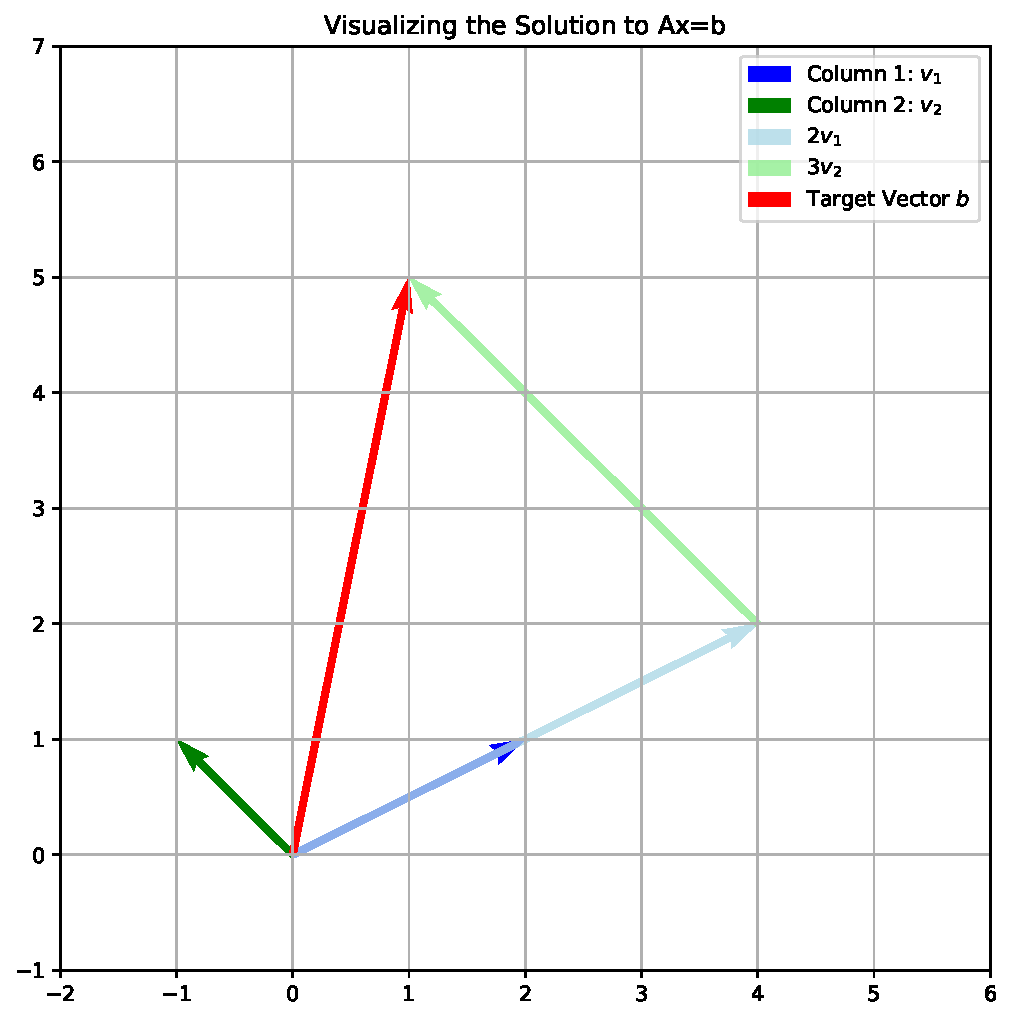
\includegraphics[keepaspectratio]{index_files/figure-pdf/fig-computational-intuition-output-1.pdf}}

}

\caption{\label{fig-computational-intuition}The Column Picture: Using
Python to see that 2 of the blue vector plus 3 of the green vector
builds the red target vector.}

\end{figure}%

By the end of this course, you won't just be able to solve these
problems. You will have a deep, visual, and computational intuition for
them. You will see a problem in your own field and recognize the
mathematical tools needed to solve it.

This course is your first and most important step towards becoming a
true architect of future technology. Let's get started.

\bookmarksetup{startatroot}

\chapter{Module-1: Linear Systems, Properties, and its
Solution}\label{module-1-linear-systems-properties-and-its-solution}

\begin{quote}
\textbf{Syllabus:} System of linear equations - Solution by Gauss
elimination - Row Echelon form and Rank of a matrix - Fundamental
theorem for linear systems of homogeneous and nonhomogeneous (statement
only) - Homogeneous linear system - Non-homogeneous linear system
\end{quote}

\bookmarksetup{startatroot}

\chapter{Introduction}\label{introduction}

Welcome! We're about to begin a journey into one of the most useful and
beautiful subjects in mathematics. But we're not going to start with
abstract definitions. We're going to start with a concrete problem that
you've seen before, but we'll look at it in a new way. The entire field
of linear algebra grew from the simple need to solve systems of linear
equations.

Let's consider a simple system:

\[
\begin{align*}
2x - y &= 1 \\
x + y &= 5
\end{align*}
\]

How do we think about this? There are two fundamental viewpoints, and
seeing them both is the key to understanding linear algebra.

\section{The Row Picture: Intersecting
Lines}\label{the-row-picture-intersecting-lines}

The first way, and the one you're probably most familiar with, is the
\textbf{Row Picture}. Each equation represents a line on the
\(xy\)-plane. The solution to the system is the single point where these
two lines intersect.

Let's use Python to see this. We're not just finding the answer; we're
visualizing the problem.

\begin{Shaded}
\begin{Highlighting}[]
\ImportTok{import}\NormalTok{ numpy }\ImportTok{as}\NormalTok{ np}
\ImportTok{import}\NormalTok{ matplotlib.pyplot }\ImportTok{as}\NormalTok{ plt}

\CommentTok{\# Define the matrix A and vector b for the system Ax = b}
\NormalTok{A }\OperatorTok{=}\NormalTok{ np.array([}
\NormalTok{    [}\DecValTok{2}\NormalTok{, }\OperatorTok{{-}}\DecValTok{1}\NormalTok{],}
\NormalTok{    [}\DecValTok{1}\NormalTok{,  }\DecValTok{1}\NormalTok{]}
\NormalTok{])}
\NormalTok{b }\OperatorTok{=}\NormalTok{ np.array([}\DecValTok{1}\NormalTok{, }\DecValTok{5}\NormalTok{])  }\CommentTok{\# Corrected}

\CommentTok{\# Solve Ax = b}
\NormalTok{solution }\OperatorTok{=}\NormalTok{ np.linalg.solve(A, b)}
\NormalTok{x\_sol, y\_sol }\OperatorTok{=}\NormalTok{ solution  }\CommentTok{\# unpack for plotting}

\CommentTok{\# For plotting the lines}
\NormalTok{x\_vals }\OperatorTok{=}\NormalTok{ np.linspace(}\DecValTok{0}\NormalTok{, }\DecValTok{4}\NormalTok{, }\DecValTok{100}\NormalTok{)}
\CommentTok{\# From 2x {-} y = 1  =\textgreater{} y = 2x {-} 1}
\NormalTok{y1\_vals }\OperatorTok{=} \DecValTok{2} \OperatorTok{*}\NormalTok{ x\_vals }\OperatorTok{{-}} \DecValTok{1}
\CommentTok{\# From x + y = 5   =\textgreater{} y = {-}x + 5}
\NormalTok{y2\_vals }\OperatorTok{=} \OperatorTok{{-}}\NormalTok{x\_vals }\OperatorTok{+} \DecValTok{5}

\CommentTok{\# {-}{-}{-} Matplotlib Plotting {-}{-}{-}}
\NormalTok{plt.figure(figsize}\OperatorTok{=}\NormalTok{(}\DecValTok{8}\NormalTok{, }\DecValTok{6}\NormalTok{))}
\NormalTok{ax }\OperatorTok{=}\NormalTok{ plt.gca()}

\CommentTok{\# Plot the two lines}
\NormalTok{ax.plot(x\_vals, y1\_vals, label}\OperatorTok{=}\StringTok{\textquotesingle{}$2x {-} y = 1$\textquotesingle{}}\NormalTok{)}
\NormalTok{ax.plot(x\_vals, y2\_vals, label}\OperatorTok{=}\StringTok{\textquotesingle{}$x + y = 5$\textquotesingle{}}\NormalTok{)}

\CommentTok{\# Plot the solution point}
\NormalTok{ax.plot(x\_sol, y\_sol, }\StringTok{\textquotesingle{}ro\textquotesingle{}}\NormalTok{, markersize}\OperatorTok{=}\DecValTok{10}\NormalTok{, label}\OperatorTok{=}\SpecialStringTok{f\textquotesingle{}Solution (}\SpecialCharTok{\{}\NormalTok{x\_sol}\SpecialCharTok{:.0f\}}\SpecialStringTok{, }\SpecialCharTok{\{}\NormalTok{y\_sol}\SpecialCharTok{:.0f\}}\SpecialStringTok{)\textquotesingle{}}\NormalTok{)}

\CommentTok{\# Titles and labels}
\NormalTok{ax.set\_title(}\StringTok{"The Row Picture"}\NormalTok{)}
\NormalTok{ax.set\_xlabel(}\StringTok{"x{-}axis"}\NormalTok{)}
\NormalTok{ax.set\_ylabel(}\StringTok{"y{-}axis"}\NormalTok{)}

\CommentTok{\# Grid, legend, limits}
\NormalTok{ax.grid(}\VariableTok{True}\NormalTok{)}
\NormalTok{ax.legend()}
\NormalTok{ax.set\_xlim(}\DecValTok{0}\NormalTok{, }\DecValTok{4}\NormalTok{)}
\NormalTok{ax.set\_ylim(}\DecValTok{0}\NormalTok{, }\DecValTok{6}\NormalTok{)}

\CommentTok{\# Show plot}
\NormalTok{plt.show()}
\end{Highlighting}
\end{Shaded}

\begin{figure}[H]

\centering{

\pandocbounded{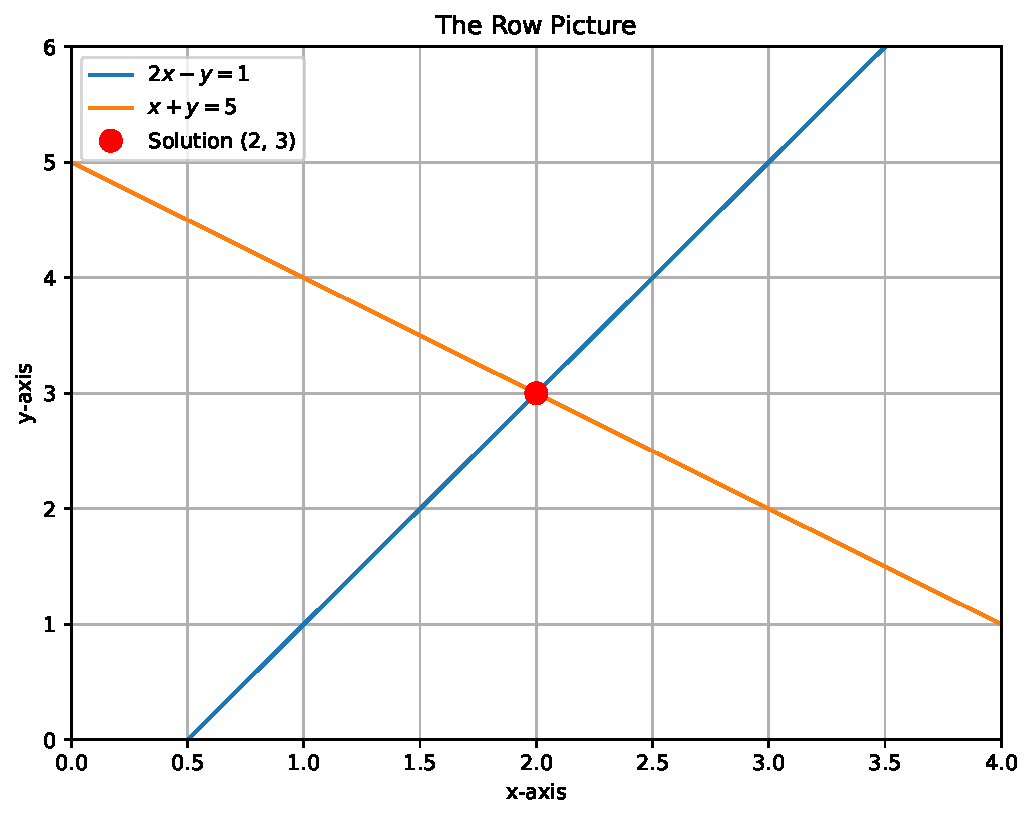
\includegraphics[keepaspectratio]{module1_files/figure-pdf/fig-row-picture-matplotlib-output-1.pdf}}

}

\caption{\label{fig-row-picture-matplotlib}The Row Picture (Matplotlib):
The solution \((2, 3)\) is the intersection of two lines.}

\end{figure}%

The plot clearly shows that the two lines meet at the point
\textbf{\((2, 3)\)}. That's our solution. For a \(3 \times 3\) system,
the row picture would be three planes intersecting at a single point.
For anything larger, we can't draw it, but the idea is the same! This is
why we need a more systematic approach.

\section{The Column Picture: Combining
Vectors}\label{the-column-picture-combining-vectors}

Now for the second way, which is completely different and incredibly
powerful. This is the \textbf{Column Picture}. We rewrite the system in
a vector form:

\[
x \begin{bmatrix} 2 \\ 1 \end{bmatrix} + y \begin{bmatrix} -1 \\ 1 \end{bmatrix} = \begin{bmatrix} 1 \\ 5 \end{bmatrix}
\]

The question now becomes: how much of the first ``column vector''
\(\begin{bmatrix} 2 \\ 1\end{bmatrix}\) do we need to add to how much of
the second ``column vector'' \(\begin{bmatrix} -1 \\ 1\end{bmatrix}\) to
get the target vector \(\begin{bmatrix} 1 \\ 5\end{bmatrix}\)?

We are trying to find the correct linear combination of the column
vectors.

Let's see what this looks like. We need to find the numbers \(x\) and
\(y\) that let us ``reach'' the target vector \(b\). From the row
picture, we already know the answer is \(x=2\) and \(y=3\). Let's verify
this with the vectors.

\begin{Shaded}
\begin{Highlighting}[]
\ImportTok{import}\NormalTok{ numpy }\ImportTok{as}\NormalTok{ np}
\ImportTok{import}\NormalTok{ matplotlib.pyplot }\ImportTok{as}\NormalTok{ plt}

\CommentTok{\# Define the vectors}
\NormalTok{v1 }\OperatorTok{=}\NormalTok{ np.array([}\DecValTok{2}\NormalTok{, }\DecValTok{1}\NormalTok{])}
\NormalTok{v2 }\OperatorTok{=}\NormalTok{ np.array([}\OperatorTok{{-}}\DecValTok{1}\NormalTok{, }\DecValTok{1}\NormalTok{])}
\NormalTok{b }\OperatorTok{=}\NormalTok{ np.array([}\DecValTok{1}\NormalTok{, }\DecValTok{5}\NormalTok{])}

\CommentTok{\# The solution coefficients}
\NormalTok{x, y }\OperatorTok{=} \DecValTok{2}\NormalTok{, }\DecValTok{3}

\CommentTok{\# Prepare the figure}
\NormalTok{plt.figure(figsize}\OperatorTok{=}\NormalTok{(}\DecValTok{6}\NormalTok{, }\DecValTok{6}\NormalTok{))}
\NormalTok{ax }\OperatorTok{=}\NormalTok{ plt.gca()}

\CommentTok{\# Draw base vectors from origin}
\NormalTok{ax.quiver(}\DecValTok{0}\NormalTok{, }\DecValTok{0}\NormalTok{, v1[}\DecValTok{0}\NormalTok{], v1[}\DecValTok{1}\NormalTok{], angles}\OperatorTok{=}\StringTok{\textquotesingle{}xy\textquotesingle{}}\NormalTok{, scale\_units}\OperatorTok{=}\StringTok{\textquotesingle{}xy\textquotesingle{}}\NormalTok{, scale}\OperatorTok{=}\DecValTok{1}\NormalTok{,}
\NormalTok{          label}\OperatorTok{=}\StringTok{\textquotesingle{}v1 = [2, 1]\textquotesingle{}}\NormalTok{)}
\NormalTok{ax.quiver(}\DecValTok{0}\NormalTok{, }\DecValTok{0}\NormalTok{, v2[}\DecValTok{0}\NormalTok{], v2[}\DecValTok{1}\NormalTok{], angles}\OperatorTok{=}\StringTok{\textquotesingle{}xy\textquotesingle{}}\NormalTok{, scale\_units}\OperatorTok{=}\StringTok{\textquotesingle{}xy\textquotesingle{}}\NormalTok{, scale}\OperatorTok{=}\DecValTok{1}\NormalTok{,}
\NormalTok{          label}\OperatorTok{=}\StringTok{\textquotesingle{}v2 = [{-}1, 1]\textquotesingle{}}\NormalTok{)}

\CommentTok{\# Draw scaled v1 (2 * v1) from origin}
\NormalTok{scaled\_v1 }\OperatorTok{=}\NormalTok{ x }\OperatorTok{*}\NormalTok{ v1}
\NormalTok{ax.quiver(}\DecValTok{0}\NormalTok{, }\DecValTok{0}\NormalTok{, scaled\_v1[}\DecValTok{0}\NormalTok{], scaled\_v1[}\DecValTok{1}\NormalTok{], angles}\OperatorTok{=}\StringTok{\textquotesingle{}xy\textquotesingle{}}\NormalTok{, scale\_units}\OperatorTok{=}\StringTok{\textquotesingle{}xy\textquotesingle{}}\NormalTok{, scale}\OperatorTok{=}\DecValTok{1}\NormalTok{,}
\NormalTok{          alpha}\OperatorTok{=}\FloatTok{0.7}\NormalTok{, label}\OperatorTok{=}\StringTok{\textquotesingle{}2 * v1\textquotesingle{}}\NormalTok{)}

\CommentTok{\# Draw scaled v2 (3 * v2) starting from the tip of 2*v1}
\NormalTok{scaled\_v2 }\OperatorTok{=}\NormalTok{ y }\OperatorTok{*}\NormalTok{ v2}
\NormalTok{ax.quiver(scaled\_v1[}\DecValTok{0}\NormalTok{], scaled\_v1[}\DecValTok{1}\NormalTok{], scaled\_v2[}\DecValTok{0}\NormalTok{], scaled\_v2[}\DecValTok{1}\NormalTok{], angles}\OperatorTok{=}\StringTok{\textquotesingle{}xy\textquotesingle{}}\NormalTok{,}
\NormalTok{          scale\_units}\OperatorTok{=}\StringTok{\textquotesingle{}xy\textquotesingle{}}\NormalTok{, scale}\OperatorTok{=}\DecValTok{1}\NormalTok{, alpha}\OperatorTok{=}\FloatTok{0.7}\NormalTok{, label}\OperatorTok{=}\StringTok{\textquotesingle{}3 * v2 (from tip of 2*v1)\textquotesingle{}}\NormalTok{)}

\CommentTok{\# Draw the target vector b from origin}
\NormalTok{ax.quiver(}\DecValTok{0}\NormalTok{, }\DecValTok{0}\NormalTok{, b[}\DecValTok{0}\NormalTok{], b[}\DecValTok{1}\NormalTok{], angles}\OperatorTok{=}\StringTok{\textquotesingle{}xy\textquotesingle{}}\NormalTok{, scale\_units}\OperatorTok{=}\StringTok{\textquotesingle{}xy\textquotesingle{}}\NormalTok{, scale}\OperatorTok{=}\DecValTok{1}\NormalTok{, color}\OperatorTok{=}\StringTok{\textquotesingle{}red\textquotesingle{}}\NormalTok{,}
\NormalTok{          label}\OperatorTok{=}\StringTok{\textquotesingle{}b = [1, 5]\textquotesingle{}}\NormalTok{)}

\CommentTok{\# Cosmetic adjustments}
\NormalTok{ax.set\_xlim(}\OperatorTok{{-}}\DecValTok{2}\NormalTok{, }\DecValTok{6}\NormalTok{)}
\NormalTok{ax.set\_ylim(}\OperatorTok{{-}}\DecValTok{2}\NormalTok{, }\DecValTok{7}\NormalTok{)}
\NormalTok{ax.set\_xlabel(}\StringTok{"x{-}component"}\NormalTok{)}
\NormalTok{ax.set\_ylabel(}\StringTok{"y{-}component"}\NormalTok{)}
\NormalTok{ax.set\_aspect(}\StringTok{\textquotesingle{}equal\textquotesingle{}}\NormalTok{, adjustable}\OperatorTok{=}\StringTok{\textquotesingle{}box\textquotesingle{}}\NormalTok{)  }\CommentTok{\# preserve vector directions/lengths}
\NormalTok{ax.grid(}\VariableTok{True}\NormalTok{)}
\NormalTok{ax.legend(loc}\OperatorTok{=}\StringTok{\textquotesingle{}upper left\textquotesingle{}}\NormalTok{)}
\NormalTok{plt.title(}\StringTok{"The Column Picture"}\NormalTok{)}
\NormalTok{plt.show()}
\end{Highlighting}
\end{Shaded}

\begin{figure}[H]

\centering{

\pandocbounded{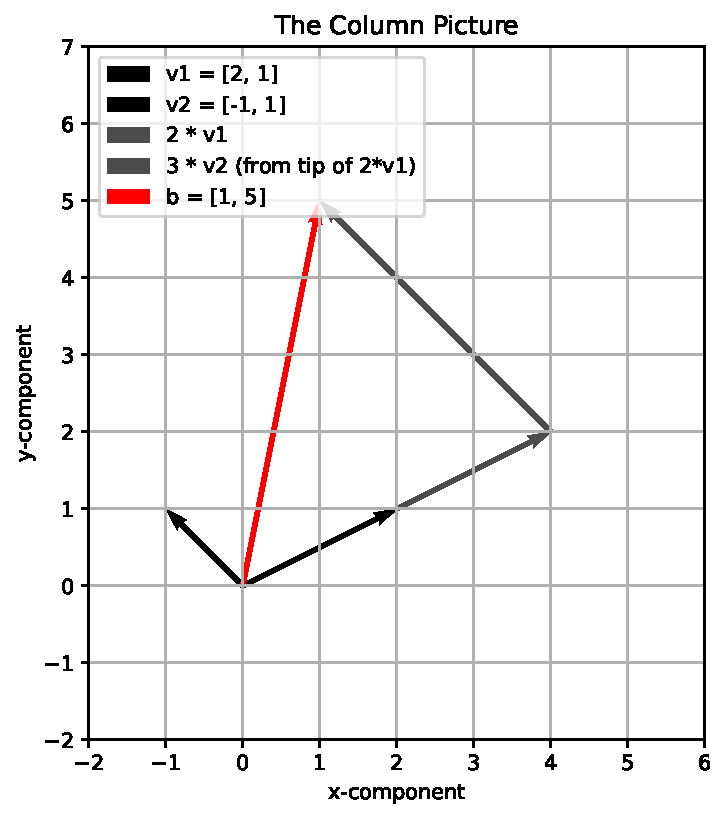
\includegraphics[keepaspectratio]{module1_files/figure-pdf/fig-column-picture-output-1.pdf}}

}

\caption{\label{fig-column-picture}The Column Picture: 2\emph{v1 + 3}v2
= b, with v1={[}2,1{]}, v2={[}-1,1{]}, b={[}1,5{]}.}

\end{figure}%

This picture shows that if you walk along the blue vector twice, and
then walk along the green vector three times, you land exactly on the
red target vector. We have found the right combination!

\section{The Algorithm: Gauss
Elimination}\label{the-algorithm-gauss-elimination}

Drawing pictures is great for intuition, but it's not a practical way to
solve a \(10 \times 10\) system. We need a rock-solid algorithm. That
algorithm is \textbf{Gauss Elimination}. The goal is simple: turn a
complicated system into a simple one that is easy to solve.

We do this by creating an \textbf{Augmented Matrix}. It's just a way to
hold all the numbers of our system without writing the variables over
and over.

For the system: \[
\begin{align*}
x + 2y + z &= 2 \\
3x + 8y + z &= 12 \\
4y + z &= 2
\end{align*}
\]

The augmented matrix is: \[
\left[
\begin{array}{ccc|c}
1 & 2 & 1 & 2 \\
3 & 8 & 1 & 12 \\
0 & 4 & 1 & 2
\end{array}
\right]
\]

\subsubsection{The Rules of the Game}\label{the-rules-of-the-game}

There are only three operations we are allowed to do. These operations
don't change the final solution: 1. Swap two rows. 2. Multiply a row by
a non-zero constant. 3. Add a multiple of one row to another row.
(\(R_i \leftarrow R_i + cR_j\))

Our goal is to use these rules to create zeros below the main diagonal.
This turns the matrix into \textbf{Row Echelon Form}.

\subsection{A Full Example: Solving a 3x3
System}\label{a-full-example-solving-a-3x3-system}

Let's solve the system above using Python's symbolic math library,
\texttt{SymPy}. This is great for teaching because it can show us the
exact steps and avoid messy decimals.

\phantomsection\label{sympy-elimination}
\begin{Shaded}
\begin{Highlighting}[]
\ImportTok{import}\NormalTok{ sympy }\ImportTok{as}\NormalTok{ sp}

\CommentTok{\# Create augmented matrix}
\NormalTok{M }\OperatorTok{=}\NormalTok{ sp.Matrix([}
\NormalTok{  [}\DecValTok{1}\NormalTok{, }\DecValTok{2}\NormalTok{, }\DecValTok{1}\NormalTok{,  }\DecValTok{2}\NormalTok{],}
\NormalTok{  [}\DecValTok{3}\NormalTok{, }\DecValTok{8}\NormalTok{, }\DecValTok{1}\NormalTok{, }\DecValTok{12}\NormalTok{],}
\NormalTok{  [}\DecValTok{0}\NormalTok{, }\DecValTok{4}\NormalTok{, }\DecValTok{1}\NormalTok{,  }\DecValTok{2}\NormalTok{]}
\NormalTok{])}

\BuiltInTok{print}\NormalTok{(}\StringTok{"Original Matrix:"}\NormalTok{)}
\NormalTok{sp.pprint(M)}

\CommentTok{\# Step 1}
\NormalTok{M[}\DecValTok{1}\NormalTok{, :] }\OperatorTok{=}\NormalTok{ M[}\DecValTok{1}\NormalTok{, :] }\OperatorTok{{-}} \DecValTok{3} \OperatorTok{*}\NormalTok{ M[}\DecValTok{0}\NormalTok{, :]}
\BuiltInTok{print}\NormalTok{(}\StringTok{"}\CharTok{\textbackslash{}n}\StringTok{After first elimination step (R\_2 \textless{}{-} R\_2 {-} 3*R\_1):"}\NormalTok{)}
\NormalTok{sp.pprint(M)}

\CommentTok{\# Step 2}
\NormalTok{M[}\DecValTok{2}\NormalTok{, :] }\OperatorTok{=}\NormalTok{ M[}\DecValTok{2}\NormalTok{, :] }\OperatorTok{{-}} \DecValTok{2} \OperatorTok{*}\NormalTok{ M[}\DecValTok{1}\NormalTok{, :]}
\BuiltInTok{print}\NormalTok{(}\StringTok{"}\CharTok{\textbackslash{}n}\StringTok{After second elimination step (R\_3 \textless{}{-} R\_3 {-} 2*R\_2):"}\NormalTok{)}
\NormalTok{sp.pprint(M)}
\end{Highlighting}
\end{Shaded}

\begin{verbatim}
Original Matrix:
⎡1  2  1  2 ⎤
⎢           ⎥
⎢3  8  1  12⎥
⎢           ⎥
⎣0  4  1  2 ⎦

After first elimination step (R_2 <- R_2 - 3*R_1):
⎡1  2  1   2⎤
⎢           ⎥
⎢0  2  -2  6⎥
⎢           ⎥
⎣0  4  1   2⎦

After second elimination step (R_3 <- R_3 - 2*R_2):
⎡1  2  1    2 ⎤
⎢             ⎥
⎢0  2  -2   6 ⎥
⎢             ⎥
⎣0  0  5   -10⎦
\end{verbatim}

Look at that final matrix! We have an upper-triangular form. This is
\textbf{Row Echelon Form}. The first non-zero entries in each row are
called \textbf{pivots}. Here our pivots are 1, 2, and 5.

The system has now become: \[
\begin{align*}
x + 2y + z &= 2 \\
2y - 2z &= 6 \\
5z &= -10
\end{align*}
\]

This is easy to solve by \emph{back substitution}. From the last row:
\(5z = -10 \implies z = -2\). Substitute into the second row:
\(2y - 2(-2) = 6 \implies 2y + 4 = 6 \implies y = 1\). Substitute both
into the first row: \(x + 2(1) + (-2) = 2 \implies x = 2\).

So the solution is \((x, y, z) = (2, 1, -2)\).

Of course, we can have a computer do this all at once. The
\texttt{rref()} method will take it all the way to \emph{Reduced Row
Echelon Form}, where the pivots are 1 and there are zeros \emph{above}
them as well.

\phantomsection\label{sympy-rref}
\begin{Shaded}
\begin{Highlighting}[]
\NormalTok{M\_original }\OperatorTok{=}\NormalTok{ sp.Matrix([}
\NormalTok{  [}\DecValTok{1}\NormalTok{, }\DecValTok{2}\NormalTok{, }\DecValTok{1}\NormalTok{,  }\DecValTok{2}\NormalTok{],}
\NormalTok{  [}\DecValTok{3}\NormalTok{, }\DecValTok{8}\NormalTok{, }\DecValTok{1}\NormalTok{, }\DecValTok{12}\NormalTok{],}
\NormalTok{  [}\DecValTok{0}\NormalTok{, }\DecValTok{4}\NormalTok{, }\DecValTok{1}\NormalTok{,  }\DecValTok{2}\NormalTok{]}
\NormalTok{])}

\NormalTok{M\_rref, pivots }\OperatorTok{=}\NormalTok{ M\_original.rref()}
\BuiltInTok{print}\NormalTok{(}\StringTok{"Reduced Row Echelon Form (RREF):"}\NormalTok{)}
\NormalTok{sp.pprint(M\_rref)}
\BuiltInTok{print}\NormalTok{(}\StringTok{"}\CharTok{\textbackslash{}n}\StringTok{Pivot columns are:"}\NormalTok{, pivots)}
\end{Highlighting}
\end{Shaded}

\begin{verbatim}
Reduced Row Echelon Form (RREF):
⎡1  0  0  2 ⎤
⎢           ⎥
⎢0  1  0  1 ⎥
⎢           ⎥
⎣0  0  1  -2⎦

Pivot columns are: (0, 1, 2)
\end{verbatim}

The RREF form directly tells us the solution: \(1x = 2\), \(1y = 1\),
\(1z = -2\).

In this method the unknowns are eliminated successively and the system
is reduced to an upper triangular system from which the unknowns can be
found by back substitution. \textgreater{}\textbf{Problem} Using Gauss
elimination method, solve the system \begin{align*}
        4x-6y &=-11\\
        -3x+8y &=10
    \end{align*}

\textbf{Solution:} The given system is \(AX=b\) where
\(A=\begin{bmatrix}
    4 &-6\\
    -3 &8
\end{bmatrix}\), \(X=\begin{bmatrix}
x\\
y
\end{bmatrix}\), \(b=\begin{bmatrix}
-11\\
10
\end{bmatrix}\) \begin{align*}
    [A|b]&=\begin{bmatrix}
        4 &-6 &\bigm| &-11\\
        -3 &8 &\bigm| &10
    \end{bmatrix}\\
&\sim \begin{bmatrix}
    4 &-6 &\bigm| &-11\\
    0 &\frac{7}{2} &\bigm| &\frac{7}{4}
\end{bmatrix}\begin{array}{c}
R_2\rightarrow R_2+\dfrac{3}{4}R_1
\end{array}
\end{align*} The system is reduced to \[\begin{bmatrix}
    4 &-6\\
    0 &\frac{7}{2}
\end{bmatrix}\begin{bmatrix}
x\\
y
\end{bmatrix}=\begin{bmatrix}
-11\\
\frac{7}{4}
\end{bmatrix}\] \begin{align*}
    4x-6y &=-11......(1)\\
    \frac{7}{2}y &=\frac{7}{4}.....(2)
\end{align*}

\((2)\rightarrow y=\frac{1}{2}\) and substituting in (1) we get
\(x=-2\). \(\therefore\) the solution is \[x=-2,y=\frac{1}{2}\]

\begin{quote}
\textbf{Problem:} Using Gauss elimination method, find the solution of
\begin{align*}
x-y &=-3\\
-2x+2y &=6
\end{align*}
\end{quote}

\textbf{Solution:} The given system is \(AX=B\) where
\(A=\begin{bmatrix}
    1 &-1\\
    -2 &2
\end{bmatrix}\), \(X=\begin{bmatrix}
    x\\
    y
\end{bmatrix}\), \(b=\begin{bmatrix}
    -3\\
    6
\end{bmatrix}\) \begin{align*}
    [A|b]&=\begin{bmatrix}
        1 &-1 &\bigm| &-3\\
        -2 &2 &\bigm| &6
    \end{bmatrix}\\
    &\sim \begin{bmatrix}
        1 &-1 &\bigm| &-3\\
        0 &0 &\bigm| &0
    \end{bmatrix}\begin{array}{c}
        R_2\rightarrow R_2+2R_1
    \end{array}
\end{align*} The system is reduced to \[\begin{bmatrix}
    1 &-1\\
    0 &0
\end{bmatrix}\begin{bmatrix}
    x\\
    y
\end{bmatrix}=\begin{bmatrix}
    -3\\
    0
\end{bmatrix}\] \begin{align*}
    x-y &=-3.....(1)\\
    0 &=0.....(2)
\end{align*}

In (1) put \(y=t\) then \(x=-3+t\). \(\therefore\) the solution is
\[x=t-3,y=t\]

\begin{quote}
\textbf{Problem} Using Gauss elimination method, find the solution of
\end{quote}

\begin{align*}
-x-y &=1\\
-3x-3y &=2
\end{align*}

\textbf{Solution:} The given system is \(AX=b\) where
\(A=\begin{bmatrix}
    -1 &-1\\
    -3 &-3
\end{bmatrix}\), \(X=\begin{bmatrix}
    x\\
    y
\end{bmatrix}\), \(b=\begin{bmatrix}
    1\\
    2
\end{bmatrix}\) \begin{align*}
    [A|b]&=\begin{bmatrix}
        -1 &-1 &\bigm| &1\\
        -3 &-3 &\bigm| &2
    \end{bmatrix}\\
    &\sim \begin{bmatrix}
        -1 &-1 &\bigm| &1\\
        0 &0 &\bigm| &-1
    \end{bmatrix}\begin{array}{c}
        R_2\rightarrow R_2-3R_1
    \end{array}
\end{align*} The system is reduced to \[\begin{bmatrix}
    -1 &-1\\
    0 &0
\end{bmatrix}\begin{bmatrix}
    x\\
    y
\end{bmatrix}=\begin{bmatrix}
    1\\
    -1
\end{bmatrix}\] \begin{align*}
    -x-y &=1.....(1)\\
    0 &=-1.....(2)
\end{align*} The false statement \(0=-1\) shows that the system has no
solution.

\begin{quote}
\textbf{Problem:} Solve the linear system \begin{align*}
x_1-x_2+x_3 &=0\\
-x_1+x_2-x_3 &=0\\
10x_2+25x_3 &= 90\\
20x_1+10x_2 &= 80
\end{align*}
\end{quote}

\textbf{Solution:} The given system is \(AX=B\) where
\(A=\begin{bmatrix}
    1 &-1 &1\\
    -1 &1 &-1\\
    0 &10 &25\\
    20 &10 &0
\end{bmatrix}\), \(X=\begin{bmatrix}
    x_1\\
    x_2\\
    x_3
\end{bmatrix}\), \(b=\begin{bmatrix}
    0\\
    0\\
    90\\
    80
\end{bmatrix}\) \begin{align*}
    [A|b]&=\begin{bmatrix}
        1 &-1  &1 &\bigm| &0\\
        -1 &1 &-1 &\bigm| &0\\
        0 &10 &25 &\bigm| &90\\
        20 &10 &0 &\bigm| &80
    \end{bmatrix}\\
    &\sim \begin{bmatrix}
        1 &-1  &1 &\bigm| &0\\
        0 &0 &0 &\bigm| &0\\
        0 &10 &25 &\bigm| &90\\
        0 &30 &-20 &\bigm| &80
    \end{bmatrix}\begin{array}{c}
        R_2\rightarrow R_2+R_1\\
        R_4\rightarrow R_4-20R_1
    \end{array}\\
    &\sim \begin{bmatrix}
    1 &-1  &1 &\bigm| &0\\
    0 &30 &-20 &\bigm| &80\\
    0 &10 &25 &\bigm| &90\\
    0 &0 &0 &\bigm| &0
\end{bmatrix}\begin{array}{c}
    R_2\leftrightarrow R_4
\end{array}\\
&\sim \begin{bmatrix}
    1 &-1  &1 &\bigm| &0\\
    0 &10 &25 &\bigm| &90\\
    0 &30 &-20 &\bigm| &80\\
        0 &0 &0 &\bigm| &0
\end{bmatrix}\begin{array}{c}
    R_2\leftrightarrow R_3
\end{array}\\
&\sim \begin{bmatrix}
    1 &-1  &1 &\bigm| &0\\
    0 &10 &25 &\bigm| &90\\
    0 &0 &-95 &\bigm| &-190\\
    0 &0 &0 &\bigm| &0
\end{bmatrix}\begin{array}{c}
    R_3\rightarrow R_3-3R_2
\end{array}\\
\end{align*} The system is reduced to \[\begin{bmatrix}
    1 &-1 &1\\
    0 &10 &25\\
    0 &0 &-95\\
    0 &0 &0
\end{bmatrix}\begin{bmatrix}
    x_1\\
    x_2\\
    x_3
\end{bmatrix}=\begin{bmatrix}
    0\\
    90\\
    -190\\
    0
\end{bmatrix}\] \begin{align*}
    x_1-x_2+x_3 &=0.....(1)\\
    10x_2+25x_3 &=90.....(2)\\
    -95x_3 &=-190........(3)\\
    0 &=0............(4)
\end{align*} \((3)\rightarrow x_3=2\) and substituting in (2), we get
\(x_2=4\)

Substituting the value of \(x_2\) and \(x_3\) in (1), we get \(x_1=2\).
\(\therefore\) the solution is \(x_1=2, x_2=4, x_3=2\).

\begin{quote}
\textbf{Problem:} Using Gauss elimination method, find the solution of
the system of equation \begin{align*}
2x+z &=3\\
x-y-z&=1\\
3x-y &= 4
\end{align*}
\end{quote}

\textbf{Solution:} The given system is \(AX=b\) where
\(A=\begin{bmatrix}
    2 &0 &1\\
    1 &-1 &-1\\
    3 &-1 &0
\end{bmatrix}\), \(X=\begin{bmatrix}
    x\\
    y\\
    z
\end{bmatrix}\), \(b=\begin{bmatrix}
    3\\
    1\\
    4
\end{bmatrix}\) \begin{align*}
    [A|b]&=\begin{bmatrix}
        2 &0  &1 &\bigm| &3\\
        1 &-1 &-1 &\bigm| &1\\
        3 &-1 &0 &\bigm| &4
    \end{bmatrix}\\
    &\sim \begin{bmatrix}
        1 &-1  &-1 &\bigm| &1\\
        2 &0 &1 &\bigm| &3\\
        3 &-1 &0 &\bigm| &4
    \end{bmatrix}\begin{array}{c}
        R_1\leftrightarrow R_2
    \end{array}\\
    &\sim \begin{bmatrix}
        1 &-1  &-1 &\bigm| &1\\
        0 &2 &3 &\bigm| &1\\
        0 &2 &3 &\bigm| &1
    \end{bmatrix}\begin{array}{c}
        R_2\rightarrow R_2-2R_1\\
        R_3\rightarrow R_3-3R_1
    \end{array}\\
    &\sim \begin{bmatrix}
        1 &-1  &-1 &\bigm| &1\\
        0 &2 &3 &\bigm| &1\\
        0 &0 &0 &\bigm| &0
    \end{bmatrix}\begin{array}{c}
        R_3\rightarrow R_3-R_2
    \end{array}
\end{align*} The system is reduced to \[\begin{bmatrix}
    1 &-1 &-1\\
    0 &2 &3\\
    0 &0 &0
\end{bmatrix}\begin{bmatrix}
    x\\
    y\\
    z
\end{bmatrix}=\begin{bmatrix}
    1\\
    1\\
    0
\end{bmatrix}\] \begin{align*}
    x-y-z &=1.....(1)\\
    2y+3z &=1.....(2)\\
    0 &=0........(3)
\end{align*} Put \(z=t\), then
\((2)\rightarrow 2y=1-3t\Rightarrow y=\frac{1}{2}-\frac{3}{2}t\)\textbackslash{}
\((1)\rightarrow x=\frac{3}{2}-\frac{1}{2}t\). \(\therefore\) the
solution is
\(x=\frac{3}{2}-\frac{1}{2}t, y=\frac{1}{2}-\frac{3}{2}t, z=t\).

\begin{quote}
\textbf{Problem:} Solve the linear system\\
\begin{align*}
3x_1+2x_2+x_3 &=3\\
2x_1+x_2+x_3 &=0\\
6x_1+2x_2+4x_3 &= 6
\end{align*}
\end{quote}

\textbf{Solution:} \$The given system is \(AX=b\) where
\(A=\begin{bmatrix}
    3 &2 &1\\
    2 &1 &1\\
    6 &2 &4
\end{bmatrix}\), \(X=\begin{bmatrix}
    x_1\\
    x_2\\
    x_3
\end{bmatrix}\), \(b=\begin{bmatrix}
    3\\
    0\\
    6
\end{bmatrix}\) \begin{align*}
    [A|b]&=\begin{bmatrix}
        3 &2  &1 &\bigm| &3\\
        2 &1 &1 &\bigm| &0\\
        6 &2 &4 &\bigm| &6
    \end{bmatrix}\\
    &\sim \begin{bmatrix}
        3 &2  &1 &\bigm| &3\\
        0 &-\frac{1}{3} &\frac{1}{3} &\bigm| &-2\\
        0 &-2 &2 &\bigm| &0
    \end{bmatrix}\begin{array}{c}
        R_2\rightarrow R_2-\frac{2}{3}R_1\\
        R_3\rightarrow R_3-2R_1
    \end{array}\\
    &\sim \begin{bmatrix}
        3 &2  &1 &\bigm| &3\\
        0 &-\frac{1}{3} &\frac{1}{3} &\bigm| &-2\\
        0 &0 &0 &\bigm| &12
    \end{bmatrix}\begin{array}{c}
        R_3\rightarrow R_3-6R_2
    \end{array}
\end{align*} The system is reduced to \[\begin{bmatrix}
    3 &2 &1\\
    0 &-\frac{1}{3} &\frac{1}{3}\\
    0 &0 &0
\end{bmatrix}\begin{bmatrix}
    x_1\\
    x_2\\
    x_3
\end{bmatrix}=\begin{bmatrix}
    3\\
    -2\\
    12
\end{bmatrix}\] \begin{align*}
    3x_1+2x_2+x_3 &=3.....(1)\\
    -\frac{1}{3}x_2+\frac{1}{3}x_3 &=9-2.....(2)\\
    0 &=12........(3)
\end{align*}

The false statement \(0=12\) shows that the system has no solution.

\begin{quote}
\textbf{Problem:} Using Gauss elimination method, find the solution of
the system of equation \begin{align*}
x+2y+z &=3\\
2x+3y+2z&=5\\
3x-5y+5z &= 2\\
3x+9y-z &=4
\end{align*}
\end{quote}

\textbf{Solution:} The given system is \(AX=B\) where
\(A=\begin{bmatrix}
    1 &2 &1\\
    2 &3 &2\\
    3 &-5 &5\\
    3 &9 &-1
\end{bmatrix}\), \(X=\begin{bmatrix}
    x\\
    y\\
    z
\end{bmatrix}\), \(b=\begin{bmatrix}
    3\\
    5\\
    2\\
    4
\end{bmatrix}\) \begin{align*}
    [A|b]&=\begin{bmatrix}
        1 &2  &1 &\bigm| &3\\
        2 &3 &2 &\bigm| &5\\
        3 &-5 &5 &\bigm| &2\\
        3 &9 &-1 &\bigm| &4
    \end{bmatrix}\\
    &\sim \begin{bmatrix}
        1 &2  &1 &\bigm| &3\\
        0 &-1 &0 &\bigm| &-1\\
        0 &-11 &2 &\bigm| &-7\\
        0 &3 &-4 &\bigm| &-5
    \end{bmatrix}\begin{array}{c}
        R_2\rightarrow R_2-2R_1\\
        R_3\rightarrow R_3-3R_1\\
        R_4\rightarrow R_4-3R_1
    \end{array}\\
    &\sim \begin{bmatrix}
        1 &2  &1 &\bigm| &3\\
        0 &-1 &0 &\bigm| &-1\\
        0 &0 &2 &\bigm| &4\\
        0 &0 &-4 &\bigm| &-8
    \end{bmatrix}\begin{array}{c}
        R_3\rightarrow R_3-11R_2\\
        R_4\rightarrow R_4+3R_2
    \end{array}\\
    &\sim \begin{bmatrix}
        1 &2  &1 &\bigm| &3\\
        0 &-1 &0 &\bigm| &-1\\
        0 &0 &2 &\bigm| &4\\
        0 &0 &0 &\bigm| &0
    \end{bmatrix}\begin{array}{c}
        R_4\rightarrow R4+2R_3
    \end{array}
\end{align*} The system is reduced to \[\begin{bmatrix}
    1 &2 &1\\
    0 &-1 &0\\
    0 &0 &2\\
    0 &0 &0
\end{bmatrix}\begin{bmatrix}
    x\\
    y\\
    z
\end{bmatrix}=\begin{bmatrix}
    3\\
    -1\\
    4\\
    0
\end{bmatrix}\] \begin{align*}
    x+2y+z &=3.....(1)\\
    -y+0z &=-1.....(2)\\
    2z &=4 .........(3)\\
    0 &=0........(4)
\end{align*} \((3)\rightarrow z=2\) and substituting in (2), we get
\(y=1\)\textbackslash{} Also substituting \(y\) and \(z\) in (1), we get
\(x=-1\). \(\therefore\) the solution is \(x=-1, y=1, z=2\).

\subsection{Row Echelon Form}\label{row-echelon-form}

At the end of the Gauss elimination the form of the coefficient matrix,
the augmented matrix and the system itself are called row echelon form.
In it, rows of zeros, if present, are the last rows and the number of
zeros before the leading nonzero element in each row is greater than the
corresponding number of zeros of the preceeding rows.

\section{Solve the following using Gauss Elimination
method.}\label{solve-the-following-using-gauss-elimination-method.}

\subsection{Question 1}\label{question-1}

Solve the system: \[
\begin{cases}
2x + y - z = 8 \\
-3x - y + 2z = -11 \\
-2x + y + 2z = -3
\end{cases}
\]

\textbf{Solution:}

Start with the augmented matrix: \[
\begin{bmatrix}
2 & 1 & -1 & 8 \\
-3 & -1 & 2 & -11 \\
-2 & 1 & 2 & -3
\end{bmatrix}
\]

Apply \(R_2 \rightarrow R_2 + \frac{3}{2}R_1\) and
\(R_3 \rightarrow R_3 + R_1\):

\[
\begin{bmatrix}
2 & 1 & -1 & 8 \\
0 & 0.5 & 0.5 & 1 \\
0 & 2 & 1 & 5
\end{bmatrix}
\]

Next, \(R_3 \rightarrow R_3 - 4R_2\):

\[
\begin{bmatrix}
2 & 1 & -1 & 8 \\
0 & 0.5 & 0.5 & 1 \\
0 & 0 & -1 & 1
\end{bmatrix}
\]

From the last row: \(z = -1\). Substituting back: - From \(R_2\):
\(0.5y + 0.5(-1) = 1 \implies y = 3\) - From \(R_1\):
\(2x + 3 - (-1) = 8 \implies x = 2\)

Final solution: \(\boxed{x=2, y=3, z=-1}\).

\begin{center}\rule{0.5\linewidth}{0.5pt}\end{center}

\subsection{Question 2}\label{question-2}

Solve: \[
\begin{cases}
x + 2y + 3z = 14 \\
2x + y + z = 10 \\
3x + 4y + 7z = 30
\end{cases}
\]

\textbf{Solution:}

Augmented matrix: \[
\begin{bmatrix}
1 & 2 & 3 & 14 \\
2 & 1 & 1 & 10 \\
3 & 4 & 7 & 30
\end{bmatrix}
\]

\(R_2 \rightarrow R_2 - 2R_1\), \(R_3 \rightarrow R_3 - 3R_1\):

\[
\begin{bmatrix}
1 & 2 & 3 & 14 \\
0 & -3 & -5 & -18 \\
0 & -2 & -2 & -12
\end{bmatrix}
\]

\(R_3 \rightarrow R_3 - \frac{2}{3}R_2\):

\[
\begin{bmatrix}
1 & 2 & 3 & 14 \\
0 & -3 & -5 & -18 \\
0 & 0 & \frac{4}{3} & 0
\end{bmatrix}
\]

From \(R_3\): \(z = 0\).\\
From \(R_2\): \(-3y - 5(0) = -18 \implies y = 6\).\\
From \(R_1\): \(x + 2(6) + 3(0) = 14 \implies x = 2\).

Solution: \(\boxed{x=2, y=6, z=0}\).

\begin{center}\rule{0.5\linewidth}{0.5pt}\end{center}

\subsection{Question 3}\label{question-3}

Solve: \[
\begin{cases}
x - y + z = 4 \\
2x + y - z = 2 \\
3x + y + z = 10
\end{cases}
\]

\textbf{Solution:}

Augmented matrix: \[
\begin{bmatrix}
1 & -1 & 1 & 4 \\
2 & 1 & -1 & 2 \\
3 & 1 & 1 & 10
\end{bmatrix}
\]

\(R_2 \rightarrow R_2 - 2R_1\), \(R_3 \rightarrow R_3 - 3R_1\):

\[
\begin{bmatrix}
1 & -1 & 1 & 4 \\
0 & 3 & -3 & -6 \\
0 & 4 & -2 & -2
\end{bmatrix}
\]

\(R_3 \rightarrow R_3 - \frac{4}{3}R_2\):

\[
\begin{bmatrix}
1 & -1 & 1 & 4 \\
0 & 3 & -3 & -6 \\
0 & 0 & 2 & 6
\end{bmatrix}
\]

From \(R_3\): \(z = 3\).\\
From \(R_2\): \(3y - 3(3) = -6 \implies y = 1\).\\
From \(R_1\): \(x - 1 + 3 = 4 \implies x = 2\).

Solution: \(\boxed{x=2, y=1, z=3}\).

\begin{center}\rule{0.5\linewidth}{0.5pt}\end{center}

\subsection{Question 4}\label{question-4}

Solve: \[
\begin{cases}
x + y + z = 6 \\
2x + 3y + 5z = 4 \\
4x + 0y + 5z = 2
\end{cases}
\]

\textbf{Solution:}

Augmented matrix: \[
\begin{bmatrix}
1 & 1 & 1 & 6 \\
2 & 3 & 5 & 4 \\
4 & 0 & 5 & 2
\end{bmatrix}
\]

\(R_2 \rightarrow R_2 - 2R_1\), \(R_3 \rightarrow R_3 - 4R_1\):

\[
\begin{bmatrix}
1 & 1 & 1 & 6 \\
0 & 1 & 3 & -8 \\
0 & -4 & 1 & -22
\end{bmatrix}
\]

\(R_3 \rightarrow R_3 + 4R_2\):

\[
\begin{bmatrix}
1 & 1 & 1 & 6 \\
0 & 1 & 3 & -8 \\
0 & 0 & 13 & -54
\end{bmatrix}
\]

From \(R_3\): \(z = -54/13\).\\
From \(R_2\):
\(y + 3(-54/13) = -8 \implies y = -8 + 162/13 = -104/13 + 162/13 = 58/13\).\\
From \(R_1\): \(x + 58/13 - 54/13 = 6 \implies x = 6 - 4/13 = 74/13\).

Solution:
\(\boxed{x=\frac{74}{13},\ y=\frac{58}{13},\ z=-\frac{54}{13}}\).

\begin{center}\rule{0.5\linewidth}{0.5pt}\end{center}

\subsection{Question 5}\label{question-5}

Solve: \[
\begin{cases}
2x + 4y - 2z = 2 \\
4x + 9y - 3z = 8 \\
-2x - 3y + 7z = 10
\end{cases}
\]

\textbf{Solution:}

Augmented matrix: \[
\begin{bmatrix}
2 & 4 & -2 & 2 \\
4 & 9 & -3 & 8 \\
-2 & -3 & 7 & 10
\end{bmatrix}
\]

\(R_2 \rightarrow R_2 - 2R_1\), \(R_3 \rightarrow R_3 + R_1\):

\[
\begin{bmatrix}
2 & 4 & -2 & 2 \\
0 & 1 & 1 & 4 \\
0 & 1 & 5 & 12
\end{bmatrix}
\]

\(R_3 \rightarrow R_3 - R_2\):

\[
\begin{bmatrix}
2 & 4 & -2 & 2 \\
0 & 1 & 1 & 4 \\
0 & 0 & 4 & 8
\end{bmatrix}
\]

From \(R_3\): \(z = 2\).\\
From \(R_2\): \(y + 2 = 4 \implies y = 2\).\\
From \(R_1\): \(2x + 8 - 4 = 2 \implies x = -1\).

Solution: \(\boxed{x=-1, y=2, z=2}\).

\section{Tutorial questions}\label{tutorial-questions}

\subsection{Problem 1: Circuit Analysis (Electronics
Core)}\label{problem-1-circuit-analysis-electronics-core}

\textbf{Scenario:}

You are given a simple DC circuit with three loops. Using Kirchhoff's
Voltage Law (KVL), which states that the sum of voltages around any
closed loop must be zero, we can set up a system of equations to find
the unknown loop currents \(i_1, i_2,\) and \(i_3\).

\begin{figure}

\centering{

\pandocbounded{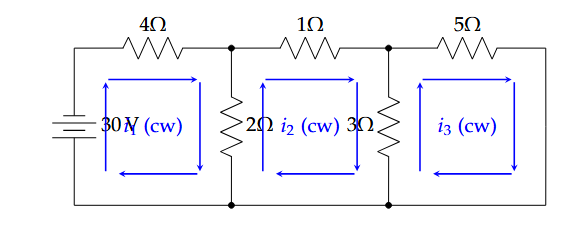
\includegraphics[keepaspectratio]{Circuit.png}}

}

\caption{\label{fig-circuit}Circuit}

\end{figure}%

\begin{itemize}
\tightlist
\item
  \textbf{Loop 1:} The 30V source minus the voltage drops across the 4Ω
  and 2Ω resistors gives the equation: \(30 - 4i_1 - 2(i_1 - i_2) = 0\)
\item
  \textbf{Loop 2:} The voltage drops across the 2Ω, 1Ω, and 3Ω resistors
  give: \(-2(i_2 - i_1) - 1i_2 - 3(i_2 - i_3) = 0\)
\item
  \textbf{Loop 3:} The voltage drops across the 3Ω and 5Ω resistors
  give: \(-3(i_3 - i_2) - 5i_3 = 0\)
\end{itemize}

Find the values of the three loop currents: \(i_1, i_2,\) and \(i_3\).

\textbf{Solution:}

\begin{quote}
Mathematical Setup
\end{quote}

First, simplify the equations and align the variables:

\begin{enumerate}
\def\labelenumi{\arabic{enumi}.}
\item
  \(30 - 6i_1 + 2i_2 = 0 \implies 6i_1 - 2i_2 + 0i_3 = 30\)
\item
  \(2i_1 - 6i_2 + 3i_3 = 0\)
\item
  \(3i_2 - 8i_3 = 0 \implies 0i_1 + 3i_2 - 8i_3 = 0\)
\end{enumerate}

This gives us the system \(Ax=b\).

\begin{quote}
Step 1: Write the Augmented Matrix \[
\left[
\begin{array}{ccc|c}
6 & -2 & 0 & 30 \\
2 & -6 & 3 & 0 \\
0 & 3 & -8 & 0
\end{array}
\right]
\]
\end{quote}

\begin{quote}
Step 2: Perform Gauss Elimination
\end{quote}

Let's simplify Row 1 first by dividing by 2: \(R_1 \leftarrow R_1 / 2\).
\[
\left[
\begin{array}{ccc|c}
3 & -1 & 0 & 15 \\
2 & -6 & 3 & 0 \\
0 & 3 & -8 & 0
\end{array}
\right]
\] Now, create a zero in the first column of Row 2. The operation is
\(R_2 \leftarrow R_2 - \frac{2}{3}R_1\). (To make it easier, let's do
\(R_2 \leftarrow 3R_2 - 2R_1\)). \[
3 \times [2, -6, 3, 0] \rightarrow [6, -18, 9, 0]
\] \[
2 \times [3, -1, 0, 15] \rightarrow [6, -2, 0, 30]
\] \[
\text{New } R_2 = [0, -16, 9, -30]
\] Our matrix is now: \[
\left[
\begin{array}{ccc|c}
3 & -1 & 0 & 15 \\
0 & -16 & 9 & -30 \\
0 & 3 & -8 & 0
\end{array}
\right]
\] Finally, let's eliminate the first element in Row 3. Oh, wait, it's
already zero! So we move to the next pivot. We need to create a zero in
the second column of Row 3. The operation is
\(R_3 \leftarrow R_3 + \frac{3}{16}R_2\) (or
\(R_3 \leftarrow 16R_3 + 3R_2\)). \[
16 \times [0, 3, -8, 0] \rightarrow [0, 48, -128, 0]
\] \[
3 \times [0, -16, 9, -30] \rightarrow [0, -48, 27, -90]
\] \[
\text{New } R_3 = [0, 0, -101, -90]
\] Our final Row Echelon Form is: \[
\left[
\begin{array}{ccc|c}
3 & -1 & 0 & 15 \\
0 & -16 & 9 & -30 \\
0 & 0 & -101 & -90
\end{array}
\right]
\]

\begin{quote}
Step 3: Back Substitution
\end{quote}

\begin{itemize}
\tightlist
\item
  From \(R_3\): \(-101i_3 = -90 \implies i_3 = 90/101 \approx 0.891\) A.
\item
  From \(R_2\):
  \(-16i_2 + 9i_3 = -30 \implies -16i_2 + 9(90/101) = -30 \implies i_2 \approx 2.375\)
  A.
\item
  From \(R_1\):
  \(3i_1 - i_2 = 15 \implies 3i_1 - 2.375 = 15 \implies i_1 \approx 5.792\)
  A.
\end{itemize}

\begin{quote}
\textbf{Python Verification}
\end{quote}

\phantomsection\label{solve-circuit}
\begin{Shaded}
\begin{Highlighting}[]
\ImportTok{import}\NormalTok{ numpy }\ImportTok{as}\NormalTok{ np}

\CommentTok{\# Coefficient matrix A (from KVL equations)}
\NormalTok{A }\OperatorTok{=}\NormalTok{ np.array([}
\NormalTok{    [}\DecValTok{6}\NormalTok{, }\OperatorTok{{-}}\DecValTok{2}\NormalTok{, }\DecValTok{0}\NormalTok{],}
\NormalTok{    [}\DecValTok{2}\NormalTok{, }\OperatorTok{{-}}\DecValTok{6}\NormalTok{, }\DecValTok{3}\NormalTok{],}
\NormalTok{    [}\DecValTok{0}\NormalTok{, }\DecValTok{3}\NormalTok{, }\OperatorTok{{-}}\DecValTok{8}\NormalTok{]}
\NormalTok{])}

\CommentTok{\# Constants vector b (from voltage sources)}
\NormalTok{b }\OperatorTok{=}\NormalTok{ np.array([}\DecValTok{30}\NormalTok{, }\DecValTok{0}\NormalTok{, }\DecValTok{0}\NormalTok{])   }\CommentTok{\# \textless{}{-}{-} adjust according to your circuit}

\CommentTok{\# Solve the system Ax = b}
\NormalTok{currents }\OperatorTok{=}\NormalTok{ np.linalg.solve(A, b)}

\BuiltInTok{print}\NormalTok{(}\StringTok{"The solution currents are:"}\NormalTok{)}
\BuiltInTok{print}\NormalTok{(}\SpecialStringTok{f"i1 = }\SpecialCharTok{\{}\NormalTok{currents[}\DecValTok{0}\NormalTok{]}\SpecialCharTok{:.3f\}}\SpecialStringTok{ Amps"}\NormalTok{)}
\BuiltInTok{print}\NormalTok{(}\SpecialStringTok{f"i2 = }\SpecialCharTok{\{}\NormalTok{currents[}\DecValTok{1}\NormalTok{]}\SpecialCharTok{:.3f\}}\SpecialStringTok{ Amps"}\NormalTok{)}
\BuiltInTok{print}\NormalTok{(}\SpecialStringTok{f"i3 = }\SpecialCharTok{\{}\NormalTok{currents[}\DecValTok{2}\NormalTok{]}\SpecialCharTok{:.3f\}}\SpecialStringTok{ Amps"}\NormalTok{)}
\end{Highlighting}
\end{Shaded}

\begin{verbatim}
The solution currents are:
i1 = 5.792 Amps
i2 = 2.376 Amps
i3 = 0.891 Amps
\end{verbatim}

\begin{center}\rule{0.5\linewidth}{0.5pt}\end{center}

\subsection{Problem 2: Polynomial Curve Fitting (Computer
Graphics)}\label{problem-2-polynomial-curve-fitting-computer-graphics}

\textbf{Scenario:} You are a game developer designing a smooth path for
a character. You want a parabola of the form \(y = ax^2 + bx + c\) to
pass through three specific points: \(P_1(-1, 10)\), \(P_2(1, 4)\), and
\(P_3(2, 7)\). Find the coefficients \(a, b,\) and \(c\) that define
this unique parabola.

\textbf{Solution}

\begin{quote}
Step 1: Mathematical Setup
\end{quote}

Each point must satisfy the equation \(y = ax^2 + bx + c\). Plugging in
the coordinates gives us three linear equations for the unknowns
\(a, b, c\).

\begin{itemize}
\tightlist
\item
  For \(P_1(-1, 10)\):
  \(a(-1)^2 + b(-1) + c = 10 \implies a - b + c = 10\)
\item
  For \(P_2(1, 4)\): \(a(1)^2 + b(1) + c = 4 \implies a + b + c = 4\)
\item
  For \(P_3(2, 7)\): \(a(2)^2 + b(2) + c = 7 \implies 4a + 2b + c = 7\)
\end{itemize}

\begin{quote}
Step 2: Gauss Elimination
\end{quote}

\begin{itemize}
\tightlist
\item
  \textbf{Matrix:}
  \(\left[ \begin{array}{ccc|c} 1 & -1 & 1 & 10 \\ 1 & 1 & 1 & 4 \\ 4 & 2 & 1 & 7 \end{array} \right]\)
\item
  \textbf{\(R_2 \leftarrow R_2 - R_1\) and
  \(R_3 \leftarrow R_3 - 4R_1\):}
  \(\left[ \begin{array}{ccc|c} 1 & -1 & 1 & 10 \\ 0 & 2 & 0 & -6 \\ 0 & 6 & -3 & -33 \end{array} \right]\)
\item
  \textbf{\(R_3 \leftarrow R_3 - 3R_2\):}
  \(\left[ \begin{array}{ccc|c} 1 & -1 & 1 & 10 \\ 0 & 2 & 0 & -6 \\ 0 & 0 & -3 & -15 \end{array} \right]\)
\end{itemize}

\begin{quote}
Step 3: Back Substitution:
\end{quote}

\begin{itemize}
\item
  \(-3c = -15 \implies c = 5\)
\item
  \(2b = -6 \implies b = -3\)
\item
  \(a - b + c = 10 \implies a - (-3) + 5 = 10 \implies a = 2\)
\item
  The parabola is \(y = 2x^2 - 3x + 5\).
\end{itemize}

\begin{quote}
\textbf{Python Verification}
\end{quote}

\begin{Shaded}
\begin{Highlighting}[]
\ImportTok{import}\NormalTok{ numpy }\ImportTok{as}\NormalTok{ np}
\ImportTok{import}\NormalTok{ matplotlib.pyplot }\ImportTok{as}\NormalTok{ plt}

\CommentTok{\# Matrix for system (x\^{}2, x, 1) at points x = {-}1, 1, 2}
\NormalTok{A }\OperatorTok{=}\NormalTok{ np.array([}
\NormalTok{    [(}\OperatorTok{{-}}\DecValTok{1}\NormalTok{)}\OperatorTok{**}\DecValTok{2}\NormalTok{, }\OperatorTok{{-}}\DecValTok{1}\NormalTok{, }\DecValTok{1}\NormalTok{],   }\CommentTok{\# point ({-}1, 10)}
\NormalTok{    [(}\DecValTok{1}\NormalTok{)}\OperatorTok{**}\DecValTok{2}\NormalTok{,  }\DecValTok{1}\NormalTok{, }\DecValTok{1}\NormalTok{],    }\CommentTok{\# point (1, 4)}
\NormalTok{    [(}\DecValTok{2}\NormalTok{)}\OperatorTok{**}\DecValTok{2}\NormalTok{,  }\DecValTok{2}\NormalTok{, }\DecValTok{1}\NormalTok{]     }\CommentTok{\# point (2, 7)}
\NormalTok{])}

\CommentTok{\# Corresponding y{-}values}
\NormalTok{b }\OperatorTok{=}\NormalTok{ np.array([}\DecValTok{10}\NormalTok{, }\DecValTok{4}\NormalTok{, }\DecValTok{7}\NormalTok{])}

\CommentTok{\# Solve for coefficients a, b, c}
\NormalTok{coeffs }\OperatorTok{=}\NormalTok{ np.linalg.solve(A, b)}
\NormalTok{a, b\_c, c }\OperatorTok{=}\NormalTok{ coeffs}

\BuiltInTok{print}\NormalTok{(}\SpecialStringTok{f"The coefficients are a=}\SpecialCharTok{\{}\NormalTok{a}\SpecialCharTok{:.1f\}}\SpecialStringTok{, b=}\SpecialCharTok{\{}\NormalTok{b\_c}\SpecialCharTok{:.1f\}}\SpecialStringTok{, c=}\SpecialCharTok{\{}\NormalTok{c}\SpecialCharTok{:.1f\}}\SpecialStringTok{"}\NormalTok{)}
\BuiltInTok{print}\NormalTok{(}\SpecialStringTok{f"The parabola is y = }\SpecialCharTok{\{}\NormalTok{a}\SpecialCharTok{:.1f\}}\SpecialStringTok{x² + }\SpecialCharTok{\{}\NormalTok{b\_c}\SpecialCharTok{:.1f\}}\SpecialStringTok{x + }\SpecialCharTok{\{}\NormalTok{c}\SpecialCharTok{:.1f\}}\SpecialStringTok{"}\NormalTok{)}

\CommentTok{\# Plotting}
\NormalTok{x\_vals }\OperatorTok{=}\NormalTok{ np.linspace(}\OperatorTok{{-}}\DecValTok{2}\NormalTok{, }\DecValTok{3}\NormalTok{, }\DecValTok{200}\NormalTok{)}
\NormalTok{y\_vals }\OperatorTok{=}\NormalTok{ a }\OperatorTok{*}\NormalTok{ x\_vals}\OperatorTok{**}\DecValTok{2} \OperatorTok{+}\NormalTok{ b\_c }\OperatorTok{*}\NormalTok{ x\_vals }\OperatorTok{+}\NormalTok{ c}

\NormalTok{plt.plot(x\_vals, y\_vals, label}\OperatorTok{=}\StringTok{\textquotesingle{}Fitted Parabola\textquotesingle{}}\NormalTok{)}
\NormalTok{plt.plot([}\OperatorTok{{-}}\DecValTok{1}\NormalTok{, }\DecValTok{1}\NormalTok{, }\DecValTok{2}\NormalTok{], [}\DecValTok{10}\NormalTok{, }\DecValTok{4}\NormalTok{, }\DecValTok{7}\NormalTok{], }\StringTok{\textquotesingle{}ro\textquotesingle{}}\NormalTok{, label}\OperatorTok{=}\StringTok{\textquotesingle{}Data Points\textquotesingle{}}\NormalTok{)}
\NormalTok{plt.legend()}
\NormalTok{plt.grid(}\VariableTok{True}\NormalTok{)}
\NormalTok{plt.show()}
\end{Highlighting}
\end{Shaded}

\begin{verbatim}
The coefficients are a=2.0, b=-3.0, c=5.0
The parabola is y = 2.0x² + -3.0x + 5.0
\end{verbatim}

\pandocbounded{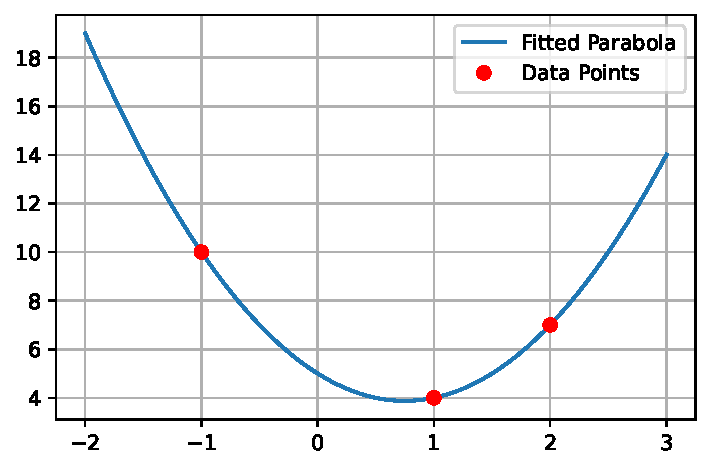
\includegraphics[keepaspectratio]{module1_files/figure-pdf/solve-polynomial-output-2.pdf}}

\begin{center}\rule{0.5\linewidth}{0.5pt}\end{center}

\subsection{Problem 3: Network Traffic Flow (Computer
Science)}\label{problem-3-network-traffic-flow-computer-science}

\textbf{Scenario:} The figure below shows the traffic flow (in cars per
hour) over a network of one-way streets. The total flow into any
intersection must equal the total flow out of that intersection. This
conservation principle gives us a system of linear equations.

\begin{figure}

\centering{

\pandocbounded{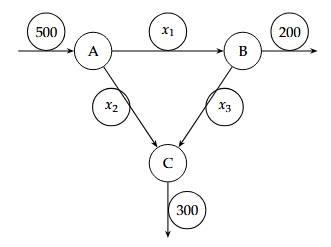
\includegraphics[keepaspectratio]{Network.png}}

}

\caption{\label{fig-network}Network diagram}

\end{figure}%

Consider a simpler 3-node network. * \textbf{Node 1:}
\(500 = x_1 + x_2\) * \textbf{Node 2:} \(x_1 + x_3 = 300\) *
\textbf{Node 3:} \(x_2 = x_3 + 200\)

Find the traffic flows \(x_1, x_2,\) and \(x_3\).

\textbf{Solution:}

\begin{quote}
Step 1: Mathematical Setup
\end{quote}

Rearrange the equations: 1. \(x_1 + x_2 + 0x_3 = 500\) 2.
\(x_1 + 0x_2 + x_3 = 300\) 3. \(0x_1 + x_2 - x_3 = 200\)

\begin{quote}
Step 2: Gauss Elimination
\end{quote}

\begin{itemize}
\item
  The matrix form of the system can be written as:
  \(\left[ \begin{array}{ccc|c} 1 & 1 & 0 & 500 \\ 1 & 0 & 1 & 300 \\ 0 & 1 & -1 & 200 \end{array} \right]\)\textbackslash{}
  Using elementory transformations;
\item
  \textbf{\(R_2 \leftarrow R_2 - R_1\):}
  \(\left[ \begin{array}{ccc|c} 1 & 1 & 0 & 500 \\ 0 & -1 & 1 & -200 \\ 0 & 1 & -1 & 200 \end{array} \right]\)
\item
  \textbf{\(R_3 \leftarrow R_3 + R_2\):}
  \(\left[ \begin{array}{ccc|c} 1 & 1 & 0 & 500 \\ 0 & -1 & 1 & -200 \\ 0 & 0 & 0 & 0 \end{array} \right]\)
\item
  It represents a system with two equations in three variables. So the
  system has infinitely many solutions!
\end{itemize}

\begin{quote}
Step 3: Back substitution
\end{quote}

From the equations; \[
\begin{cases}
x_1 + x_2 = 500 \\
x_2 - x_3 = 200
\end{cases}
\]

Let \(x_3 = t\) (free parameter). Then:

\[
x_2 = 200 + t, \quad 
x_1 = 500 - x_2 = 300 - t.
\]

Thus the solution set is:

\[
(x_1, x_2, x_3) = (300 - t,\; 200 + t,\; t), \qquad t \in \mathbb{R}.
\]

\begin{center}\rule{0.5\linewidth}{0.5pt}\end{center}

\begin{quote}
\emph{Non-Negative Constraints}
\end{quote}

If the variables represent flows, they must satisfy \(x_i \geq 0\):

\[
\begin{align*}
x_1 &= 300 - t \geq 0 \quad \Rightarrow \quad t \leq 300\\
x_2 &= 200 + t \geq 0 \quad \Rightarrow \quad t \geq -200\\
x_3 = t \geq 0
\end{align*}
\] Hence the valid range is: \[
0 \leq t \leq 300
\]

\begin{center}\rule{0.5\linewidth}{0.5pt}\end{center}

\emph{Example Solution}

For \(t = 50\), we get one solution as given below:

\[
(x_1, x_2, x_3) = (250, 250, 50).
\]

\begin{quote}
\emph{Python code for verification}
\end{quote}

\phantomsection\label{solve-traffic}
\begin{Shaded}
\begin{Highlighting}[]
\ImportTok{import}\NormalTok{ numpy }\ImportTok{as}\NormalTok{ np}

\CommentTok{\# Coefficient matrix from the equations:}
\CommentTok{\# x1 + x2      = 500}
\CommentTok{\# x1     + x3  = 300}
\CommentTok{\#      x2 {-} x3 = 200}
\NormalTok{A }\OperatorTok{=}\NormalTok{ np.array([}
\NormalTok{    [}\DecValTok{1}\NormalTok{, }\DecValTok{1}\NormalTok{, }\DecValTok{0}\NormalTok{],}
\NormalTok{    [}\DecValTok{1}\NormalTok{, }\DecValTok{0}\NormalTok{, }\DecValTok{1}\NormalTok{],}
\NormalTok{    [}\DecValTok{0}\NormalTok{, }\DecValTok{1}\NormalTok{, }\OperatorTok{{-}}\DecValTok{1}\NormalTok{]}
\NormalTok{])}
\NormalTok{b }\OperatorTok{=}\NormalTok{ np.array([}\DecValTok{500}\NormalTok{, }\DecValTok{300}\NormalTok{, }\DecValTok{200}\NormalTok{])}

\CommentTok{\# Since this system is dependent, use least{-}squares solution}
\NormalTok{flows, residuals, rank, s }\OperatorTok{=}\NormalTok{ np.linalg.lstsq(A, b, rcond}\OperatorTok{=}\VariableTok{None}\NormalTok{)}

\NormalTok{x1, x2, x3 }\OperatorTok{=}\NormalTok{ flows}

\BuiltInTok{print}\NormalTok{(}\StringTok{"General traffic flow solution (with free variable t):"}\NormalTok{)}
\BuiltInTok{print}\NormalTok{(}\SpecialStringTok{f"x1 = }\SpecialCharTok{\{}\NormalTok{x1}\SpecialCharTok{:.1f\}}\SpecialStringTok{ + t"}\NormalTok{)}
\BuiltInTok{print}\NormalTok{(}\SpecialStringTok{f"x2 = }\SpecialCharTok{\{}\NormalTok{x2}\SpecialCharTok{:.1f\}}\SpecialStringTok{ {-} t"}\NormalTok{)}
\BuiltInTok{print}\NormalTok{(}\SpecialStringTok{f"x3 = }\SpecialCharTok{\{}\NormalTok{x3}\SpecialCharTok{:.1f\}}\SpecialStringTok{ + t"}\NormalTok{)}
\end{Highlighting}
\end{Shaded}

\begin{verbatim}
General traffic flow solution (with free variable t):
x1 = 266.7 + t
x2 = 233.3 - t
x3 = 33.3 + t
\end{verbatim}

\section{Rank and The Fundamental
Theorem}\label{rank-and-the-fundamental-theorem}

The number of pivots in a matrix is a fundamentally important number. It
is called the \textbf{Rank} of the matrix.

\begin{quote}
\textbf{Definition: Rank} The rank of a matrix \(A\) is the number of
pivots in its row echelon form.
\end{quote}

In our example, the rank is 3. The rank cannot be larger than the number
of rows or columns.

This brings us to the \emph{Fundamental Theorem for Linear Systems}.
This theorem tells us everything about the existence and uniqueness of
solutions.

\begin{quote}
\textbf{The Fundamental Theorem for Linear Systems (Statement Only)}

\begin{enumerate}
\def\labelenumi{\arabic{enumi}.}
\item
  \textbf{Existence:} A system \(Ax = b\) has a solution if and only if
  the rank of the coefficient matrix \(A\) is equal to the rank of the
  augmented matrix \([A | b]\). (In other words, the elimination process
  doesn't lead to an impossible equation like \(0 = 5\)).
\item
  \textbf{Uniqueness:}

  \begin{itemize}
  \tightlist
  \item
    If a solution exists and the
    \(\text{rank} = \text{number of variables}\), the solution is
    \emph{unique}.
  \item
    If a solution exists and the
    \(\text{rank} < \text{number of variables}\), there are
    \emph{infinitely many solutions}. The difference
    \((\text{number of variables} - \text{rank})\) tells you the number
    of ``free variables'' you can choose.
  \end{itemize}
\end{enumerate}
\end{quote}

\section{Problems on Rank of a
Matrix}\label{problems-on-rank-of-a-matrix}

\subsection{Problem 1}\label{problem-1}

Find the rank of
\(A = \begin{bmatrix} 1 & 2 & 3 \\ 2 & 4 & 6 \\ 3 & 6 & 9 \end{bmatrix}.\)

\textbf{Solution:}\\
Applying row operations: \[
R_2 \to R_2 - 2R_1, \quad R_3 \to R_3 - 3R_1
\] \[
\Rightarrow \begin{bmatrix} 1 & 2 & 3 \\ 0 & 0 & 0 \\ 0 & 0 & 0 \end{bmatrix}
\] Only one non-zero row remains.\\
\textbf{Rank = 1}.

\begin{center}\rule{0.5\linewidth}{0.5pt}\end{center}

\subsection{Problem 2}\label{problem-2}

Find the rank of
\(B = \begin{bmatrix} 2 & 4 & 1 \\ 0 & 5 & 2 \\ 0 & 0 & 3 \end{bmatrix}.\)

\textbf{Solution:}\\
The matrix is in upper triangular form. All diagonal entries are
non-zero.\\
\textbf{Rank = 3}.

\begin{center}\rule{0.5\linewidth}{0.5pt}\end{center}

\subsection{Problem 3}\label{problem-3}

Find the rank of
\(C = \begin{bmatrix} 1 & 1 & 1 \\ 1 & 2 & 3 \\ 1 & 3 & 6 \end{bmatrix}.\)

\textbf{Solution:}\\
Applying \(R_2 \to R_2 - R_1\) and \(R_3 \to R_3 - R_1\): \[
\Rightarrow \begin{bmatrix} 1 & 1 & 1 \\ 0 & 1 & 2 \\ 0 & 2 & 5 \end{bmatrix}
\] Now \(R_3 \to R_3 - 2R_2\): \[
\Rightarrow \begin{bmatrix} 1 & 1 & 1 \\ 0 & 1 & 2 \\ 0 & 0 & 1 \end{bmatrix}
\] All rows are non-zero.\\
\textbf{Rank = 3}.

\begin{center}\rule{0.5\linewidth}{0.5pt}\end{center}

\subsection{Problem 4}\label{problem-4}

Find the rank of
\(D = \begin{bmatrix} 1 & 2 & 3 & 4 \\ 2 & 4 & 6 & 8 \\ 1 & 3 & 4 & 7 \end{bmatrix}.\)

\textbf{Solution:}

\(R_2 \to R_2 - 2R_1\), \(R_3 \to R_3 - R_1\): \[
\Rightarrow \begin{bmatrix} 1 & 2 & 3 & 4 \\ 0 & 0 & 0 & 0 \\ 0 & 1 & 1 & 3 \end{bmatrix}
\] Swap \(R_2\) and \(R_3\): \[
\Rightarrow \begin{bmatrix} 1 & 2 & 3 & 4 \\ 0 & 1 & 1 & 3 \\ 0 & 0 & 0 & 0 \end{bmatrix}
\] Two non-zero rows.\\
\textbf{Rank = 2}.

\begin{center}\rule{0.5\linewidth}{0.5pt}\end{center}

\subsection{Problem 5}\label{problem-5}

Find the rank of
\(A = \begin{bmatrix} 0 & 2 & 4 \\ 1 & 3 & 5 \\ 2 & 4 & 6 \end{bmatrix}.\)

\textbf{Solution:}\\
Swap \(R_1\) and \(R_2\): \[
\Rightarrow \begin{bmatrix} 1 & 3 & 5 \\ 0 & 2 & 4 \\ 2 & 4 & 6 \end{bmatrix}
\] \(R_3 \to R_3 - 2R_1\): \[
\Rightarrow \begin{bmatrix} 1 & 3 & 5 \\ 0 & 2 & 4 \\ 0 & -2 & -4 \end{bmatrix}
\] \(R_3 \to R_3 + R_2\): \[
\Rightarrow \begin{bmatrix} 1 & 3 & 5 \\ 0 & 2 & 4 \\ 0 & 0 & 0 \end{bmatrix}
\] Two non-zero rows.\\
\textbf{Rank = 2}.

\section{Application problems}\label{application-problems}

\subsection{Problem 1}\label{problem-1-1}

In a digital communication system, three transmitted signals are
received at three different antennas. The received signal strengths (in
arbitrary units) are represented by the matrix, \[
A =
\begin{bmatrix}
2 & 3 & 1 \\
4 & 6 & 2 \\
1 & 1.5 & 0.5
\end{bmatrix}
\]

Determine the rank of \(A\) and comment on whether the received signals
are linearly independent.

\textbf{Solution:}\\
By performing Gaussian elimination: \[
R_2 \to R_2 - 2R_1,\quad R_3 \to R_3 - 0.5R_1
\] We get:

\[
\begin{bmatrix}
2 & 3 & 1 \\
0 & 0 & 0 \\
0 & 0 & 0
\end{bmatrix}
\]

The rank is \$1\$. This implies that all received signals are linearly
dependent --- effectively carrying the same information.

\begin{center}\rule{0.5\linewidth}{0.5pt}\end{center}

\subsection{Problem 2}\label{problem-2-1}

In a computer vision system, the transformation matrix mapping 3D world
points to 2D image points is given by:

\[
B =
\begin{bmatrix}
1 & 0 & 2 \\
0 & 1 & 3 \\
2 & 1 & 7
\end{bmatrix}
\]

Find the rank of \(B\) and state whether the transformation is
invertible.

\textbf{Solution:}\\
Perform:

\[
R_3 \to R_3 - 2R_1
\]

\[
\begin{bmatrix}
1 & 0 & 2 \\
0 & 1 & 3 \\
0 & 1 & 3
\end{bmatrix}
\]

Now:

\[
R_3 \to R_3 - R_2
\]

\[
\begin{bmatrix}
1 & 0 & 2 \\
0 & 1 & 3 \\
0 & 0 & 0
\end{bmatrix}
\]

Rank = \(2\). The transformation is not invertible because it is not
full rank.

\begin{center}\rule{0.5\linewidth}{0.5pt}\end{center}

\subsection{Problem 3}\label{problem-3-1}

In a microprocessor system, the current equations for three loops are
given by:

\[
\begin{cases}
2I_1 + I_2 + I_3 = 5 \\
4I_1 + 2I_2 + 2I_3 = 10 \\
3I_1 + 1.5I_2 + 1.5I_3 = 7.5
\end{cases}
\]

Form the coefficient matrix and determine its rank. Comment on the
uniqueness of the solution.

\textbf{Solution:}\\
Coefficient matrix:

\[
C =
\begin{bmatrix}
2 & 1 & 1 \\
4 & 2 & 2 \\
3 & 1.5 & 1.5
\end{bmatrix}
\]

Using Gaussian elimination, all rows become proportional to the first
row, giving rank = \(1\).\\
Since the rank is less than the number of variables, the system has
infinitely many solutions.

\begin{center}\rule{0.5\linewidth}{0.5pt}\end{center}

\subsection{Problem 4}\label{problem-4-1}

In a data transmission system, the coding matrix is:

\[
D =
\begin{bmatrix}
1 & 2 & 3 & 4 \\
2 & 4 & 6 & 8 \\
1 & 3 & 4 & 7
\end{bmatrix}
\]

Find the rank and explain its implication on error detection capability.

\textbf{Solution:}\\
Perform:

\[
R_2 \to R_2 - 2R_1
\]

\[
\begin{bmatrix}
1 & 2 & 3 & 4 \\
0 & 0 & 0 & 0 \\
1 & 3 & 4 & 7
\end{bmatrix}
\]

\[
R_3 \to R_3 - R_1
\]

\[
\begin{bmatrix}
1 & 2 & 3 & 4 \\
0 & 0 & 0 & 0 \\
0 & 1 & 1 & 3
\end{bmatrix}
\]

This has two non-zero rows → rank = \(2\).\\
A rank less than the number of columns implies reduced ability to detect
and correct transmission errors.

\begin{center}\rule{0.5\linewidth}{0.5pt}\end{center}

\subsection{Problem 5}\label{problem-5-1}

An image compression algorithm stores pixel blocks as linear
combinations of a set of basis images. The matrix of basis images is:

\[
E =
\begin{bmatrix}
1 & 0 & 1 \\
0 & 1 & 1 \\
1 & 1 & 2
\end{bmatrix}
\]

Find the rank of \(E\) and comment on whether the basis set is minimal.

\textbf{Solution:}\\
Perform: \[
R_3 \to R_3 - R_1
\]

\[
\begin{bmatrix}
1 & 0 & 1 \\
0 & 1 & 1 \\
0 & 1 & 1
\end{bmatrix}
\]

\[
R_3 \to R_3 - R_2
\]

\[
\begin{bmatrix}
1 & 0 & 1 \\
0 & 1 & 1 \\
0 & 0 & 0
\end{bmatrix}
\]

Rank = \(2\). This means the third basis image is not independent; a
smaller basis can be used for compression.

\section{Homogeneous and Non-Homogeneous
Systems}\label{homogeneous-and-non-homogeneous-systems}

There are two main flavors of systems we need to discuss.

\subsection{\texorpdfstring{Homogeneous System:
\(Ax = 0\)}{Homogeneous System: Ax = 0}}\label{homogeneous-system-ax-0}

This is a system where the right-hand side is all zeros. For example:
\(x + 2y + z = 0\).

\begin{itemize}
\tightlist
\item
  These systems \emph{always} have at least one solution: the
  \emph{trivial solution} \(x=0, y=0, z=0\).
\item
  The interesting question is whether they have \emph{non-trivial}
  solutions.
\item
  From the Fundamental Theorem, we will have infinitely many
  (non-trivial) solutions if
  \(\text{rank} < \text{number of variables}\). The solutions form a
  space called the \emph{nullspace}.
\end{itemize}

Let's find the nullspace of a different matrix, one that has a
non-trivial nullspace.

\phantomsection\label{sympy-nullspace}
\begin{Shaded}
\begin{Highlighting}[]
\ImportTok{import}\NormalTok{ sympy }\ImportTok{as}\NormalTok{ sp}

\CommentTok{\# Matrix with non{-}trivial nullspace}
\NormalTok{B }\OperatorTok{=}\NormalTok{ sp.Matrix([}
\NormalTok{  [}\DecValTok{1}\NormalTok{, }\DecValTok{2}\NormalTok{, }\DecValTok{3}\NormalTok{],}
\NormalTok{  [}\DecValTok{4}\NormalTok{, }\DecValTok{5}\NormalTok{, }\DecValTok{6}\NormalTok{],}
\NormalTok{  [}\DecValTok{7}\NormalTok{, }\DecValTok{8}\NormalTok{, }\DecValTok{9}\NormalTok{]}
\NormalTok{])}

\NormalTok{nullspace\_vectors }\OperatorTok{=}\NormalTok{ B.nullspace()}
\BuiltInTok{print}\NormalTok{(}\SpecialStringTok{f"The rank of matrix B is }\SpecialCharTok{\{}\NormalTok{B}\SpecialCharTok{.}\NormalTok{rank()}\SpecialCharTok{\}}\SpecialStringTok{. It has }\SpecialCharTok{\{}\NormalTok{B}\SpecialCharTok{.}\NormalTok{shape[}\DecValTok{1}\NormalTok{]}\SpecialCharTok{\}}\SpecialStringTok{ columns."}\NormalTok{)}
\BuiltInTok{print}\NormalTok{(}\StringTok{"The nullspace is spanned by:"}\NormalTok{)}
\NormalTok{sp.pprint(nullspace\_vectors)}
\end{Highlighting}
\end{Shaded}

\begin{verbatim}
The rank of matrix B is 2. It has 3 columns.
The nullspace is spanned by:
⎡⎡1 ⎤⎤
⎢⎢  ⎥⎥
⎢⎢-2⎥⎥
⎢⎢  ⎥⎥
⎣⎣1 ⎦⎦
\end{verbatim}

For matrix \(B\), the rank (2) is less than the number of variables (3),
so there is one free variable and the nullspace is a line through the
origin. Any multiple of the vector \([1, -2, 1]^T\) is a solution to
\(Bx=0\).

\subsection{\texorpdfstring{Non-Homogeneous System:
\(Ax = b\)}{Non-Homogeneous System: Ax = b}}\label{non-homogeneous-system-ax-b}

This is the general case where \(b\) is not all zeros. The complete
solution has a beautiful structure.

\begin{quote}
\emph{Structure of the Complete Solution} The complete solution to
\(Ax = b\) is given by:
\[ x_{\text{complete}} = x_{\text{particular}} + x_{\text{homogeneous}} \]

Where: * \(x_{\text{particular}}\) is \textbf{one} particular solution
to \(Ax = b\). * \(x_{\text{homogeneous}}\) is \textbf{all} the
solutions to the associated homogeneous system \(Ax = 0\).
\end{quote}

This is an amazing and deep result! It says that the set of all
solutions to \(Ax = b\) is just a shifted version of the nullspace. The
nullspace goes through the origin, and we just shift the whole thing by
one particular solution vector.

\section{Module I Summary}\label{module-i-summary}

\begin{itemize}
\tightlist
\item
  We can view a linear system in two ways: the \emph{Row Picture}
  (intersecting hyperplanes) and the \emph{Column Picture} (linear
  combination of vectors).
\item
  \emph{Gauss Elimination} is the core algorithm for solving any system.
  It reduces the system to \emph{Row Echelon Form}.
\item
  The \emph{rank} of a matrix is the number of pivots, and it's the most
  important number about that matrix.
\item
  The \emph{Fundamental Theorem} tells us when solutions exist and if
  they are unique, all based on the rank.
\item
  The complete solution to \(Ax = b\) is a combination of one particular
  solution and all solutions to \(Ax = 0\) (the nullspace).
\end{itemize}

This module has set the stage. We have the main problem (\(Ax=b\)) and
the main algorithm (elimination). In the next modules, we will build a
much deeper understanding of the matrix \(A\) itself.

\bookmarksetup{startatroot}

\chapter{Module-2: Matrix Eigen Value
Problems}\label{module-2-matrix-eigen-value-problems}

\begin{quote}
\textbf{Syllabus:} Eigen values and Eigen vectors - Properties of Eigen
values - Diagonalization of matrices - Orthogonal transformation and
orthogonal matrices - Quadratic forms and their Canonical forms.
\end{quote}

\section{\texorpdfstring{The Big Question: What Does a Matrix
\emph{Do}?}{The Big Question: What Does a Matrix Do?}}\label{the-big-question-what-does-a-matrix-do}

In the first module, we treated matrices as simple containers for the
numbers in a linear system. But a matrix is much more than that. A
matrix is a \emph{transformation}. It takes a vector and maps it to a
new vector.

When you multiply a vector \(x\) by a matrix \(A\), the resulting vector
\(Ax\) is usually stretched and rotated. It points in a new direction.

But for any given matrix, there are a few very special vectors. When you
multiply these special vectors by the matrix, they \textbf{do not change
direction}. They only get stretched or shrunk. The output vector \(Ax\)
is parallel to the input vector \(x\).

These special vectors are the \textbf{eigenvectors} of the matrix, and
the scaling factor is the \textbf{eigenvalue}.

\begin{quote}
\textbf{Definition: Eigenvalue and Eigenvector} For a square matrix
\(A\), a non-zero vector \(x\) is an eigenvector if it satisfies the
equation: \[ Ax = \lambda x \] where \(\lambda\) is a scalar known as
the eigenvalue corresponding to the eigenvector \(x\).
\end{quote}

The eigenvectors tell you the ``axes'' of the transformation, the
directions that are preserved. The eigenvalues tell you the scaling
factor along those axes. If you know the eigenvalues and eigenvectors of
a matrix, you understand its fundamental behavior.

\section{Finding Eigenvalues and
Eigenvectors}\label{finding-eigenvalues-and-eigenvectors}

How do we find these special numbers \(\lambda\) and vectors \(x\)? We
start by rewriting the main equation.

\[
\begin{align*}
Ax &= \lambda x \\
Ax - \lambda x &= 0 \\
Ax - \lambda I x &= 0 && \text{(where I is the identity matrix)} \\
(A - \lambda I)x &= 0
\end{align*}
\]

Look at that last line! It's a homogeneous system of equations, just
like we saw in Module I. We are looking for a \emph{non-zero} solution
for \(x\). For the system \((A - \lambda I)x = 0\) to have a non-trivial
solution, the matrix \((A - \lambda I)\) must be \textbf{singular}.

And what does it mean for a matrix to be singular? Its determinant must
be zero.

\begin{quote}
\textbf{The Characteristic Equation} \[ \det(A - \lambda I) = 0 \]
\end{quote}

Solving this equation for \(\lambda\) gives us the eigenvalues. Then,
for each eigenvalue, we plug it back into \((A - \lambda I)x = 0\) to
find the corresponding eigenvector(s).

\begin{tcolorbox}[enhanced jigsaw, colframe=quarto-callout-note-color-frame, coltitle=black, bottomtitle=1mm, toptitle=1mm, toprule=.15mm, leftrule=.75mm, rightrule=.15mm, breakable, title=\textcolor{quarto-callout-note-color}{\faInfo}\hspace{0.5em}{Shortcut for finding eigen values of 2x2 Matrices}, left=2mm, opacityback=0, titlerule=0mm, arc=.35mm, bottomrule=.15mm, opacitybacktitle=0.6, colbacktitle=quarto-callout-note-color!10!white, colback=white]

For any 2x2 matrix \(A = \begin{bmatrix} a & b \\ c & d \end{bmatrix}\),
the characteristic equation is always:
\[ \lambda^2 - (\text{trace}(A))\lambda + \det(A) = 0 \] Where:

\begin{itemize}
\item
  The \textbf{trace} is the sum of the diagonal elements:
  \(\text{trace}(A) = a+d\).
\item
  The \textbf{determinant} is \(\det(A) = ad-bc\).
\end{itemize}

This is a beautiful and powerful result! You don't need to calculate
\(\det(A - \lambda I)\) from scratch; just find the trace and
determinant and plug them into the quadratic formula.

\end{tcolorbox}

\begin{tcolorbox}[enhanced jigsaw, colframe=quarto-callout-note-color-frame, coltitle=black, bottomtitle=1mm, toptitle=1mm, toprule=.15mm, leftrule=.75mm, rightrule=.15mm, breakable, title=\textcolor{quarto-callout-note-color}{\faInfo}\hspace{0.5em}{Shortcut for finding eigen values of 3x3 Matrices}, left=2mm, opacityback=0, titlerule=0mm, arc=.35mm, bottomrule=.15mm, opacitybacktitle=0.6, colbacktitle=quarto-callout-note-color!10!white, colback=white]

A similar, though more complex, shortcut exists for 3x3 matrices. The
characteristic equation is:
\[ \lambda^3 - (\text{trace}(A))\lambda^2 + C\lambda - \det(A) = 0 \]
Where \(C\) is the sum of the determinants of the 2x2 principal minors
(the matrices you get by deleting the \(i\)-th row and \(i\)-th column).
\[ C = \det\begin{pmatrix} a_{22} & a_{23} \\ a_{32} & a_{33} \end{pmatrix} + \det\begin{pmatrix} a_{11} & a_{13} \\ a_{31} & a_{33} \end{pmatrix} + \det\begin{pmatrix} a_{11} & a_{12} \\ a_{21} & a_{22} \end{pmatrix} \]
While this formula works, solving a cubic equation can be difficult, and
this is where numerical methods often become more practical.

\end{tcolorbox}

\subsection{Example: A Symbolic
Approach}\label{example-a-symbolic-approach}

Let's do this for a simple matrix
\(A = \begin{bmatrix} 4 & -2 \\ 1 & 1 \end{bmatrix}\) using
\texttt{SymPy} to see all the steps.

\phantomsection\label{find-eigenvalues-symbolic}
\begin{Shaded}
\begin{Highlighting}[]
\ImportTok{import}\NormalTok{ sympy }\ImportTok{as}\NormalTok{ sp}

\CommentTok{\# Define our matrix A}
\NormalTok{A }\OperatorTok{=}\NormalTok{ sp.Matrix([}
\NormalTok{    [}\DecValTok{4}\NormalTok{, }\OperatorTok{{-}}\DecValTok{2}\NormalTok{],}
\NormalTok{    [}\DecValTok{1}\NormalTok{,  }\DecValTok{1}\NormalTok{]}
\NormalTok{])}

\CommentTok{\# Create a symbol for lambda}
\NormalTok{lam }\OperatorTok{=}\NormalTok{ sp.symbols(}\StringTok{\textquotesingle{}lambda\textquotesingle{}}\NormalTok{)}

\CommentTok{\# Create the Identity matrix of the same size as A}
\NormalTok{I }\OperatorTok{=}\NormalTok{ sp.eye(A.shape[}\DecValTok{0}\NormalTok{])  }\CommentTok{\# Corrected}

\CommentTok{\# Form the matrix (A {-} lambda*I)}
\NormalTok{char\_matrix }\OperatorTok{=}\NormalTok{ A }\OperatorTok{{-}}\NormalTok{ lam }\OperatorTok{*}\NormalTok{ I}

\BuiltInTok{print}\NormalTok{(}\StringTok{"The matrix (A {-} λI):"}\NormalTok{)}
\NormalTok{sp.pprint(char\_matrix)}

\CommentTok{\# Calculate the determinant to get the characteristic polynomial}
\NormalTok{char\_poly }\OperatorTok{=}\NormalTok{ char\_matrix.det()}
\BuiltInTok{print}\NormalTok{(}\SpecialStringTok{f"}\CharTok{\textbackslash{}n}\SpecialStringTok{The characteristic polynomial det(A {-} λI) is: }\SpecialCharTok{\{}\NormalTok{char\_poly}\SpecialCharTok{\}}\SpecialStringTok{"}\NormalTok{)}

\CommentTok{\# Solve the characteristic equation det(A {-} λI) = 0 for the eigenvalues}
\NormalTok{eigenvalues }\OperatorTok{=}\NormalTok{ sp.solve(char\_poly, lam)}
\BuiltInTok{print}\NormalTok{(}\SpecialStringTok{f"}\CharTok{\textbackslash{}n}\SpecialStringTok{The eigenvalues are: }\SpecialCharTok{\{}\NormalTok{eigenvalues}\SpecialCharTok{\}}\SpecialStringTok{"}\NormalTok{)}

\CommentTok{\# SymPy can also do this in one step}
\BuiltInTok{print}\NormalTok{(}\StringTok{"}\CharTok{\textbackslash{}n}\StringTok{{-}{-}{-} Using SymPy\textquotesingle{}s built{-}in function {-}{-}{-}"}\NormalTok{)}
\NormalTok{sp.pprint(A.eigenvects())}
\end{Highlighting}
\end{Shaded}

\begin{verbatim}
The matrix (A - λI):
⎡4 - λ   -2  ⎤
⎢            ⎥
⎣  1    1 - λ⎦

The characteristic polynomial det(A - λI) is: lambda**2 - 5*lambda + 6

The eigenvalues are: [2, 3]

--- Using SymPy's built-in function ---
⎡⎛      ⎡⎡1⎤⎤⎞  ⎛      ⎡⎡2⎤⎤⎞⎤
⎢⎜2, 1, ⎢⎢ ⎥⎥⎟, ⎜3, 1, ⎢⎢ ⎥⎥⎟⎥
⎣⎝      ⎣⎣1⎦⎦⎠  ⎝      ⎣⎣1⎦⎦⎠⎦
\end{verbatim}

The output shows that for our matrix \(A\), the eigenvalues are
\(\lambda_1 = 3\) and \(\lambda_2 = 2\). The corresponding eigenvectors
are multiples of \(\begin{bmatrix} 2 \\ 1 \end{bmatrix}\) and
\(\begin{bmatrix} 1 \\ 1 \end{bmatrix}\).

\subsection{Key Properties of
Eigenvalues}\label{key-properties-of-eigenvalues}

The shortcuts above hint at a deeper connection. Here are the most
important properties of eigenvalues for any \(n \times n\) matrix \(A\).

\begin{itemize}
\tightlist
\item
  \textbf{Sum:} The sum of the eigenvalues is equal to the trace of the
  matrix. \[ \sum_{i=1}^{n} \lambda_i = \text{trace}(A) \]
\item
  \textbf{Product:} The product of the eigenvalues is equal to the
  determinant of the matrix. \[ \prod_{i=1}^{n} \lambda_i = \det(A) \]
\item
  \textbf{Singularity:} A matrix is singular (not invertible) if and
  only if at least one of its eigenvalues is zero. (This follows
  directly from the product property).
\item
  \textbf{Powers:} The eigenvalues of \(A^k\) are
  \(\lambda_1^k, \lambda_2^k, \dots, \lambda_n^k\).
\item
  \textbf{Inverse:} The eigenvalues of \(A^{-1}\) are
  \(1/\lambda_1, 1/\lambda_2, \dots, 1/\lambda_n\).
\item
  \textbf{Transpose:} A matrix and its transpose, \(A\) and \(A^T\),
  have the same eigenvalues.
\item
  \textbf{Triangular Matrices:} The eigenvalues of a triangular (or
  diagonal) matrix are simply the entries on its main diagonal.
\end{itemize}

Let's verify a few of these properties with code.

\phantomsection\label{verify-properties}
\begin{Shaded}
\begin{Highlighting}[]
\ImportTok{import}\NormalTok{ numpy }\ImportTok{as}\NormalTok{ np}

\CommentTok{\# A sample 3x3 matrix}
\NormalTok{A }\OperatorTok{=}\NormalTok{ np.array([}
\NormalTok{    [}\DecValTok{2}\NormalTok{, }\DecValTok{1}\NormalTok{, }\OperatorTok{{-}}\DecValTok{1}\NormalTok{],}
\NormalTok{    [}\DecValTok{6}\NormalTok{, }\OperatorTok{{-}}\DecValTok{1}\NormalTok{, }\DecValTok{0}\NormalTok{],}
\NormalTok{    [}\OperatorTok{{-}}\DecValTok{1}\NormalTok{, }\OperatorTok{{-}}\DecValTok{2}\NormalTok{, }\OperatorTok{{-}}\DecValTok{1}\NormalTok{]}
\NormalTok{])}

\CommentTok{\# Get the eigenvalues using NumPy}
\NormalTok{eigenvalues }\OperatorTok{=}\NormalTok{ np.linalg.eigvals(A)}

\BuiltInTok{print}\NormalTok{(}\SpecialStringTok{f"The matrix A is:}\CharTok{\textbackslash{}n}\SpecialCharTok{\{}\NormalTok{A}\SpecialCharTok{\}}\SpecialStringTok{"}\NormalTok{)}
\BuiltInTok{print}\NormalTok{(}\SpecialStringTok{f"}\CharTok{\textbackslash{}n}\SpecialStringTok{Its eigenvalues are: }\SpecialCharTok{\{}\NormalTok{eigenvalues}\SpecialCharTok{\}}\SpecialStringTok{"}\NormalTok{)}

\CommentTok{\# Verify the Sum property}
\NormalTok{sum\_of\_eigenvalues }\OperatorTok{=}\NormalTok{ np.}\BuiltInTok{sum}\NormalTok{(eigenvalues)}
\NormalTok{trace\_of\_A }\OperatorTok{=}\NormalTok{ np.trace(A)}
\BuiltInTok{print}\NormalTok{(}\SpecialStringTok{f"}\CharTok{\textbackslash{}n}\SpecialStringTok{Sum of eigenvalues: }\SpecialCharTok{\{}\NormalTok{sum\_of\_eigenvalues}\SpecialCharTok{:.4f\}}\SpecialStringTok{"}\NormalTok{)}
\BuiltInTok{print}\NormalTok{(}\SpecialStringTok{f"Trace of A: }\SpecialCharTok{\{}\NormalTok{trace\_of\_A}\SpecialCharTok{\}}\SpecialStringTok{"}\NormalTok{)}
\BuiltInTok{print}\NormalTok{(}\SpecialStringTok{f"Are they close? }\SpecialCharTok{\{}\NormalTok{np}\SpecialCharTok{.}\NormalTok{isclose(sum\_of\_eigenvalues, trace\_of\_A)}\SpecialCharTok{\}}\SpecialStringTok{"}\NormalTok{)}

\CommentTok{\# Verify the Product property}
\NormalTok{product\_of\_eigenvalues }\OperatorTok{=}\NormalTok{ np.prod(eigenvalues)}
\NormalTok{determinant\_of\_A }\OperatorTok{=}\NormalTok{ np.linalg.det(A)}
\BuiltInTok{print}\NormalTok{(}\SpecialStringTok{f"}\CharTok{\textbackslash{}n}\SpecialStringTok{Product of eigenvalues: }\SpecialCharTok{\{}\NormalTok{product\_of\_eigenvalues}\SpecialCharTok{:.4f\}}\SpecialStringTok{"}\NormalTok{)}
\BuiltInTok{print}\NormalTok{(}\SpecialStringTok{f"Determinant of A: }\SpecialCharTok{\{}\NormalTok{determinant\_of\_A}\SpecialCharTok{:.4f\}}\SpecialStringTok{"}\NormalTok{)}
\BuiltInTok{print}\NormalTok{(}\SpecialStringTok{f"Are they close? }\SpecialCharTok{\{}\NormalTok{np}\SpecialCharTok{.}\NormalTok{isclose(product\_of\_eigenvalues, determinant\_of\_A)}\SpecialCharTok{\}}\SpecialStringTok{"}\NormalTok{)}
\end{Highlighting}
\end{Shaded}

\begin{verbatim}
The matrix A is:
[[ 2  1 -1]
 [ 6 -1  0]
 [-1 -2 -1]]

Its eigenvalues are: [ 3.91899444+0.j         -1.95949722+1.23243177j -1.95949722-1.23243177j]

Sum of eigenvalues: 0.0000+0.0000j
Trace of A: 0
Are they close? True

Product of eigenvalues: 21.0000+0.0000j
Determinant of A: 21.0000
Are they close? True
\end{verbatim}

\subsection{Example: Finding Eigenvectors by
Hand}\label{example-finding-eigenvectors-by-hand}

Now that we have the eigenvalues, how do we find the eigenvectors? We
solve the system \((A - \lambda I)x = 0\). Let's do this for our first
example, \(A = \begin{bmatrix} 4 & -2 \\ 1 & 1 \end{bmatrix}\), where we
found \(\lambda_1 = 3\) and \(\lambda_2 = 2\).

\textbf{Case 1: Find eigenvector for \(\lambda_1 = 3\).}

We need to solve \((A - 3I)x = 0\).
\[ (A - 3I) = \begin{bmatrix} 4-3 & -2 \\ 1 & 1-3 \end{bmatrix} = \begin{bmatrix} 1 & -2 \\ 1 & -2 \end{bmatrix} \]
So the system is:
\[ \begin{bmatrix} 1 & -2 \\ 1 & -2 \end{bmatrix} \begin{bmatrix} x_1 \\ x_2 \end{bmatrix} = \begin{bmatrix} 0 \\ 0 \end{bmatrix} \]
Both rows give the same equation: \(x_1 - 2x_2 = 0\), or \(x_1 = 2x_2\).
This system has a free variable! If we choose \(x_2 = 1\), then
\(x_1 = 2\). So our eigenvector is a multiple of
\(v_1 = \begin{bmatrix} 2 \\ 1 \end{bmatrix}\).

\textbf{Case 2: Find eigenvector for \(\lambda_2 = 2\).}

We need to solve \((A - 2I)x = 0\).
\[ (A - 2I) = \begin{bmatrix} 4-2 & -2 \\ 1 & 1-2 \end{bmatrix} = \begin{bmatrix} 2 & -2 \\ 1 & -1 \end{bmatrix} \]
The system is \(2x_1 - 2x_2 = 0\), or \(x_1 = x_2\). If we choose
\(x_2=1\), then \(x_1=1\). So our eigenvector is a multiple of
\(v_2 = \begin{bmatrix} 1 \\ 1 \end{bmatrix}\).

These match the results we get from our computer programs perfectly!

\section{The Geometry of
Eigenvectors}\label{the-geometry-of-eigenvectors}

Let's visualize what the matrix \(A\) does to the plane. We will take a
circle of vectors, apply the matrix \(A\) to each one, and see where
they land. The circle will be transformed into an ellipse.

The key thing to watch for is that the eigenvectors lie along the axes
of this new ellipse. They are the only vectors that don't get rotated
off their original line.

\begin{Shaded}
\begin{Highlighting}[]
\ImportTok{import}\NormalTok{ numpy }\ImportTok{as}\NormalTok{ np}
\ImportTok{import}\NormalTok{ matplotlib.pyplot }\ImportTok{as}\NormalTok{ plt}

\CommentTok{\# Define the matrix A}
\NormalTok{A }\OperatorTok{=}\NormalTok{ np.array([}
\NormalTok{    [}\DecValTok{4}\NormalTok{, }\OperatorTok{{-}}\DecValTok{2}\NormalTok{],}
\NormalTok{    [}\DecValTok{1}\NormalTok{,  }\DecValTok{1}\NormalTok{]}
\NormalTok{])}

\CommentTok{\# Get eigenvalues and eigenvectors}
\NormalTok{eigvals, eigvecs }\OperatorTok{=}\NormalTok{ np.linalg.eig(A)}
\NormalTok{v1 }\OperatorTok{=}\NormalTok{ eigvecs[:, }\DecValTok{0}\NormalTok{]}
\NormalTok{v2 }\OperatorTok{=}\NormalTok{ eigvecs[:, }\DecValTok{1}\NormalTok{]}

\CommentTok{\# Create a unit circle}
\NormalTok{theta }\OperatorTok{=}\NormalTok{ np.linspace(}\DecValTok{0}\NormalTok{, }\DecValTok{2}\OperatorTok{*}\NormalTok{np.pi, }\DecValTok{200}\NormalTok{)}
\NormalTok{circle\_vectors }\OperatorTok{=}\NormalTok{ np.array([np.cos(theta), np.sin(theta)])}

\CommentTok{\# Transform the circle into an ellipse}
\NormalTok{transformed\_vectors }\OperatorTok{=}\NormalTok{ A }\OperatorTok{@}\NormalTok{ circle\_vectors}

\CommentTok{\# {-}{-}{-} Plot {-}{-}{-}}
\NormalTok{fig, ax }\OperatorTok{=}\NormalTok{ plt.subplots(figsize}\OperatorTok{=}\NormalTok{(}\DecValTok{6}\NormalTok{, }\DecValTok{6}\NormalTok{))}

\CommentTok{\# Original circle (blue)}
\NormalTok{ax.plot(circle\_vectors[}\DecValTok{0}\NormalTok{, :], circle\_vectors[}\DecValTok{1}\NormalTok{, :], color}\OperatorTok{=}\StringTok{\textquotesingle{}blue\textquotesingle{}}\NormalTok{, label}\OperatorTok{=}\StringTok{\textquotesingle{}Original Circle\textquotesingle{}}\NormalTok{)}

\CommentTok{\# Transformed ellipse (green)}
\NormalTok{ax.plot(transformed\_vectors[}\DecValTok{0}\NormalTok{, :], transformed\_vectors[}\DecValTok{1}\NormalTok{, :], color}\OperatorTok{=}\StringTok{\textquotesingle{}green\textquotesingle{}}\NormalTok{, label}\OperatorTok{=}\StringTok{\textquotesingle{}Transformed Ellipse\textquotesingle{}}\NormalTok{)}

\CommentTok{\# Eigenvectors transformed (red dashed) — scaled by eigenvalues}
\NormalTok{ax.plot([}\DecValTok{0}\NormalTok{, eigvals[}\DecValTok{0}\NormalTok{] }\OperatorTok{*}\NormalTok{ v1[}\DecValTok{0}\NormalTok{]], [}\DecValTok{0}\NormalTok{, eigvals[}\DecValTok{0}\NormalTok{] }\OperatorTok{*}\NormalTok{ v1[}\DecValTok{1}\NormalTok{]], }\StringTok{\textquotesingle{}r{-}{-}\textquotesingle{}}\NormalTok{, linewidth}\OperatorTok{=}\DecValTok{2}\NormalTok{, label}\OperatorTok{=}\SpecialStringTok{f\textquotesingle{}Eigenvector λ=}\SpecialCharTok{\{}\NormalTok{eigvals[}\DecValTok{0}\NormalTok{]}\SpecialCharTok{:.2f\}}\SpecialStringTok{\textquotesingle{}}\NormalTok{)}
\NormalTok{ax.plot([}\DecValTok{0}\NormalTok{, eigvals[}\DecValTok{1}\NormalTok{] }\OperatorTok{*}\NormalTok{ v2[}\DecValTok{0}\NormalTok{]], [}\DecValTok{0}\NormalTok{, eigvals[}\DecValTok{1}\NormalTok{] }\OperatorTok{*}\NormalTok{ v2[}\DecValTok{1}\NormalTok{]], }\StringTok{\textquotesingle{}r{-}{-}\textquotesingle{}}\NormalTok{, linewidth}\OperatorTok{=}\DecValTok{2}\NormalTok{, label}\OperatorTok{=}\SpecialStringTok{f\textquotesingle{}Eigenvector λ=}\SpecialCharTok{\{}\NormalTok{eigvals[}\DecValTok{1}\NormalTok{]}\SpecialCharTok{:.2f\}}\SpecialStringTok{\textquotesingle{}}\NormalTok{)}

\CommentTok{\# Formatting}
\NormalTok{ax.set\_aspect(}\StringTok{\textquotesingle{}equal\textquotesingle{}}\NormalTok{, adjustable}\OperatorTok{=}\StringTok{\textquotesingle{}box\textquotesingle{}}\NormalTok{)}
\NormalTok{ax.set\_xlim(}\OperatorTok{{-}}\DecValTok{5}\NormalTok{, }\DecValTok{5}\NormalTok{)}
\NormalTok{ax.set\_ylim(}\OperatorTok{{-}}\DecValTok{5}\NormalTok{, }\DecValTok{5}\NormalTok{)}
\NormalTok{ax.set\_xlabel(}\StringTok{\textquotesingle{}X{-}axis\textquotesingle{}}\NormalTok{)}
\NormalTok{ax.set\_ylabel(}\StringTok{\textquotesingle{}Y{-}axis\textquotesingle{}}\NormalTok{)}
\NormalTok{ax.set\_title(}\StringTok{\textquotesingle{}Geometric Action of a Matrix\textquotesingle{}}\NormalTok{)}
\NormalTok{ax.legend()}
\NormalTok{ax.grid(}\VariableTok{True}\NormalTok{)}

\NormalTok{plt.show()}
\end{Highlighting}
\end{Shaded}

\begin{figure}[H]

\centering{

\pandocbounded{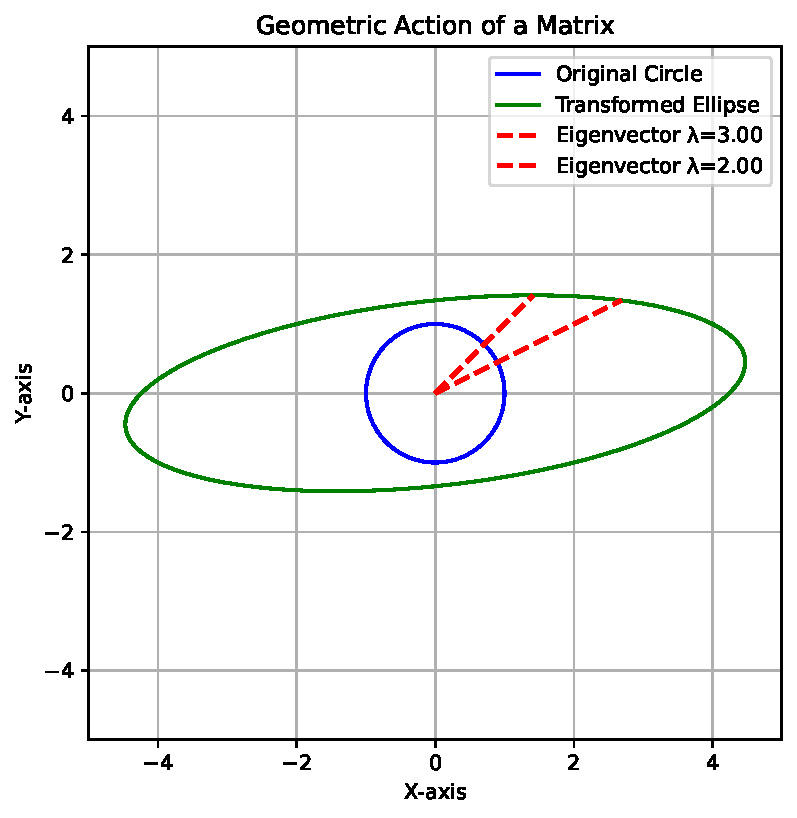
\includegraphics[keepaspectratio]{module2_files/figure-pdf/fig-eigenvector-geometry-output-1.pdf}}

}

\caption{\label{fig-eigenvector-geometry}The unit circle (blue) is
transformed into an ellipse (green). The eigenvectors (red) only
stretch, keeping their direction.}

\end{figure}%

\section{Diagonalization of a Matrix}\label{diagonalization-of-a-matrix}

This brings us to one of the most powerful ideas in linear algebra:
\textbf{diagonalization}. The goal is to write a matrix \(A\) as a
product of three simpler matrices.

\begin{quote}
\textbf{The Diagonalization Formula} \[ A = S \Lambda S^{-1} \] Where: *
\(S\) is the matrix whose columns are the eigenvectors of \(A\). *
\(\Lambda\) (Lambda) is the diagonal matrix with the eigenvalues on its
diagonal.
\end{quote}

A matrix can be diagonalized if and only if it has a full set of
linearly independent eigenvectors.

Why is this so useful? Consider computing \(A^{100}\). This would be a
nightmare. But if \(A\) is diagonalized:
\[ A^2 = (S \Lambda S^{-1})(S \Lambda S^{-1}) = S \Lambda (S^{-1}S) \Lambda S^{-1} = S \Lambda^2 S^{-1} \]
In general: \[ A^k = S \Lambda^k S^{-1} \] Computing \(\Lambda^k\) is
trivial: you just raise the diagonal entries to the \(k\)-th power!

\subsection{Example: Verifying
Diagonalization}\label{example-verifying-diagonalization}

Let's verify \(A = S \Lambda S^{-1}\) and compute \(A^3\) for our
matrix.

\phantomsection\label{verify-diagonalization}
\begin{Shaded}
\begin{Highlighting}[]
\ImportTok{import}\NormalTok{ numpy }\ImportTok{as}\NormalTok{ np}

\CommentTok{\# Our matrix A}
\NormalTok{A }\OperatorTok{=}\NormalTok{ np.array([}
\NormalTok{    [}\DecValTok{4}\NormalTok{, }\OperatorTok{{-}}\DecValTok{2}\NormalTok{],}
\NormalTok{    [}\DecValTok{1}\NormalTok{,  }\DecValTok{1}\NormalTok{]}
\NormalTok{], dtype}\OperatorTok{=}\BuiltInTok{float}\NormalTok{)  }\CommentTok{\# ensure float for safety in inverse}

\CommentTok{\# NumPy\textquotesingle{}s eig function gives both eigenvalues and eigenvectors}
\NormalTok{eigenvalues, eigenvectors }\OperatorTok{=}\NormalTok{ np.linalg.eig(A)}

\CommentTok{\# S is the matrix of eigenvectors}
\NormalTok{S }\OperatorTok{=}\NormalTok{ eigenvectors}
\CommentTok{\# Λ is the diagonal matrix of eigenvalues}
\NormalTok{Lambda }\OperatorTok{=}\NormalTok{ np.diag(eigenvalues)}

\BuiltInTok{print}\NormalTok{(}\StringTok{"Matrix S (Eigenvectors):"}\NormalTok{)}
\BuiltInTok{print}\NormalTok{(S)}
\BuiltInTok{print}\NormalTok{(}\StringTok{"}\CharTok{\textbackslash{}n}\StringTok{Matrix Λ (Eigenvalues):"}\NormalTok{)}
\BuiltInTok{print}\NormalTok{(Lambda)}

\CommentTok{\# Calculate S{-}inverse}
\NormalTok{S\_inv }\OperatorTok{=}\NormalTok{ np.linalg.inv(S)}

\CommentTok{\# Verify A = SΛS⁻¹}
\NormalTok{A\_reconstructed }\OperatorTok{=}\NormalTok{ S }\OperatorTok{@}\NormalTok{ Lambda }\OperatorTok{@}\NormalTok{ S\_inv}
\BuiltInTok{print}\NormalTok{(}\StringTok{"}\CharTok{\textbackslash{}n}\StringTok{Reconstructed A = SΛS⁻¹:"}\NormalTok{)}
\BuiltInTok{print}\NormalTok{(A\_reconstructed)}
\BuiltInTok{print}\NormalTok{(}\StringTok{"}\CharTok{\textbackslash{}n}\StringTok{Is it close to the original A?"}\NormalTok{, np.allclose(A, A\_reconstructed))}

\CommentTok{\# Compute A³ directly}
\NormalTok{A\_cubed\_direct }\OperatorTok{=}\NormalTok{ np.linalg.matrix\_power(A, }\DecValTok{3}\NormalTok{)}

\CommentTok{\# Compute A³ using diagonalization}
\NormalTok{Lambda\_cubed }\OperatorTok{=}\NormalTok{ np.diag(eigenvalues}\OperatorTok{**}\DecValTok{3}\NormalTok{)}
\NormalTok{A\_cubed\_diagonal }\OperatorTok{=}\NormalTok{ S }\OperatorTok{@}\NormalTok{ Lambda\_cubed }\OperatorTok{@}\NormalTok{ S\_inv}

\BuiltInTok{print}\NormalTok{(}\StringTok{"}\CharTok{\textbackslash{}n}\StringTok{{-}{-}{-} Computing A³ {-}{-}{-}"}\NormalTok{)}
\BuiltInTok{print}\NormalTok{(}\StringTok{"Direct computation (A³):"}\NormalTok{)}
\BuiltInTok{print}\NormalTok{(A\_cubed\_direct)}
\BuiltInTok{print}\NormalTok{(}\StringTok{"}\CharTok{\textbackslash{}n}\StringTok{Using diagonalization (SΛ³S⁻¹):"}\NormalTok{)}
\BuiltInTok{print}\NormalTok{(A\_cubed\_diagonal)}
\BuiltInTok{print}\NormalTok{(}\StringTok{"}\CharTok{\textbackslash{}n}\StringTok{Are the results close?"}\NormalTok{, np.allclose(A\_cubed\_direct, A\_cubed\_diagonal))}
\end{Highlighting}
\end{Shaded}

\begin{verbatim}
Matrix S (Eigenvectors):
[[0.89442719 0.70710678]
 [0.4472136  0.70710678]]

Matrix Λ (Eigenvalues):
[[3. 0.]
 [0. 2.]]

Reconstructed A = SΛS⁻¹:
[[ 4. -2.]
 [ 1.  1.]]

Is it close to the original A? True

--- Computing A³ ---
Direct computation (A³):
[[ 46. -38.]
 [ 19. -11.]]

Using diagonalization (SΛ³S⁻¹):
[[ 46. -38.]
 [ 19. -11.]]

Are the results close? True
\end{verbatim}

\section{Symmetric and Orthogonal
Matrices}\label{symmetric-and-orthogonal-matrices}

Things get even nicer for a very special class of matrices:
\textbf{symmetric matrices}, where \(A = A^T\).

Symmetric matrices have two incredible properties: 1. All their
eigenvalues are real numbers. 2. Their eigenvectors can be chosen to be
\textbf{orthogonal} (perpendicular to each other).

If we normalize the eigenvectors (make them unit length), they form an
\textbf{orthonormal set}. The matrix \(Q\) whose columns are these
orthonormal eigenvectors is an \textbf{orthogonal matrix}.

Orthogonal matrices are wonderful because their inverse is simply their
transpose: \(Q^{-1} = Q^T\).

This leads to the \textbf{Spectral Theorem}, which says that any
symmetric matrix can be diagonalized as: \[ A = Q \Lambda Q^T \]

\section{Application: Quadratic
Forms}\label{application-quadratic-forms}

What are these ideas good for? One classic application is understanding
the geometry of \textbf{quadratic forms}. A quadratic form is a
polynomial where every term has degree two. For example:
\[ f(x, y) = 2x^2 + 6xy + 2y^2 \] This equation describes a shape on the
plane. But what shape? The \(6xy\) ``cross-product'' term makes it hard
to see because it corresponds to a rotated shape. Our goal is to
eliminate this term.

We can write any quadratic form using a symmetric matrix:
\[ f(x, y) = \begin{bmatrix} x & y \end{bmatrix} \begin{bmatrix} 2 & 3 \\ 3 & 2 \end{bmatrix} \begin{bmatrix} x \\ y \end{bmatrix} = x^T A x \]

The eigenvectors of \(A\) point along the principal axes of the shape,
and the eigenvalues tell us the scaling in those directions. By changing
to a coordinate system aligned with the eigenvectors, we can describe
the shape without a cross-term.

Let's find the axes of the ellipse given by \(2x^2 + 6xy + 2y^2 = 1\).

\begin{Shaded}
\begin{Highlighting}[]
\ImportTok{import}\NormalTok{ numpy }\ImportTok{as}\NormalTok{ np}
\ImportTok{import}\NormalTok{ matplotlib.pyplot }\ImportTok{as}\NormalTok{ plt}

\CommentTok{\# Symmetric matrix for the quadratic form}
\NormalTok{A }\OperatorTok{=}\NormalTok{ np.array([}
\NormalTok{    [}\DecValTok{3}\NormalTok{, }\DecValTok{1}\NormalTok{],}
\NormalTok{    [}\DecValTok{1}\NormalTok{, }\DecValTok{2}\NormalTok{]}
\NormalTok{])}

\CommentTok{\# Eigen{-}decomposition gives the axes and scaling}
\NormalTok{eigvals, eigvecs }\OperatorTok{=}\NormalTok{ np.linalg.eig(A)}
\NormalTok{v1 }\OperatorTok{=}\NormalTok{ eigvecs[:, }\DecValTok{0}\NormalTok{]}
\NormalTok{v2 }\OperatorTok{=}\NormalTok{ eigvecs[:, }\DecValTok{1}\NormalTok{]}

\CommentTok{\# Generate grid data}
\NormalTok{x }\OperatorTok{=}\NormalTok{ np.linspace(}\OperatorTok{{-}}\FloatTok{1.5}\NormalTok{, }\FloatTok{1.5}\NormalTok{, }\DecValTok{400}\NormalTok{)}
\NormalTok{y }\OperatorTok{=}\NormalTok{ np.linspace(}\OperatorTok{{-}}\FloatTok{1.5}\NormalTok{, }\FloatTok{1.5}\NormalTok{, }\DecValTok{400}\NormalTok{)}
\NormalTok{X, Y }\OperatorTok{=}\NormalTok{ np.meshgrid(x, y)}

\CommentTok{\# Quadratic form value: F(x, y) = [x y] A [x; y]}
\NormalTok{F }\OperatorTok{=}\NormalTok{ A[}\DecValTok{0}\NormalTok{, }\DecValTok{0}\NormalTok{] }\OperatorTok{*}\NormalTok{ X}\OperatorTok{**}\DecValTok{2} \OperatorTok{+} \DecValTok{2} \OperatorTok{*}\NormalTok{ A[}\DecValTok{0}\NormalTok{, }\DecValTok{1}\NormalTok{] }\OperatorTok{*}\NormalTok{ X }\OperatorTok{*}\NormalTok{ Y }\OperatorTok{+}\NormalTok{ A[}\DecValTok{1}\NormalTok{, }\DecValTok{1}\NormalTok{] }\OperatorTok{*}\NormalTok{ Y}\OperatorTok{**}\DecValTok{2}

\CommentTok{\# Plotting}
\NormalTok{plt.figure(figsize}\OperatorTok{=}\NormalTok{(}\DecValTok{7}\NormalTok{, }\DecValTok{7}\NormalTok{))}

\CommentTok{\# Draw the level set F = 1 (ellipse)}
\NormalTok{plt.contour(X, Y, F, levels}\OperatorTok{=}\NormalTok{[}\DecValTok{1}\NormalTok{], colors}\OperatorTok{=}\StringTok{\textquotesingle{}blue\textquotesingle{}}\NormalTok{)}

\CommentTok{\# Draw eigenvectors scaled by semi{-}axis lengths}
\NormalTok{axis1 }\OperatorTok{=}\NormalTok{ v1 }\OperatorTok{/}\NormalTok{ np.sqrt(eigvals[}\DecValTok{0}\NormalTok{])}
\NormalTok{axis2 }\OperatorTok{=}\NormalTok{ v2 }\OperatorTok{/}\NormalTok{ np.sqrt(eigvals[}\DecValTok{1}\NormalTok{])}

\NormalTok{plt.quiver(}\DecValTok{0}\NormalTok{, }\DecValTok{0}\NormalTok{, axis1[}\DecValTok{0}\NormalTok{], axis1[}\DecValTok{1}\NormalTok{], angles}\OperatorTok{=}\StringTok{\textquotesingle{}xy\textquotesingle{}}\NormalTok{, scale\_units}\OperatorTok{=}\StringTok{\textquotesingle{}xy\textquotesingle{}}\NormalTok{, scale}\OperatorTok{=}\DecValTok{1}\NormalTok{, color}\OperatorTok{=}\StringTok{\textquotesingle{}red\textquotesingle{}}\NormalTok{, label}\OperatorTok{=}\SpecialStringTok{f\textquotesingle{}Axis 1 (λ=}\SpecialCharTok{\{}\NormalTok{eigvals[}\DecValTok{0}\NormalTok{]}\SpecialCharTok{:.2f\}}\SpecialStringTok{)\textquotesingle{}}\NormalTok{)}
\NormalTok{plt.quiver(}\DecValTok{0}\NormalTok{, }\DecValTok{0}\NormalTok{, }\OperatorTok{{-}}\NormalTok{axis1[}\DecValTok{0}\NormalTok{], }\OperatorTok{{-}}\NormalTok{axis1[}\DecValTok{1}\NormalTok{], angles}\OperatorTok{=}\StringTok{\textquotesingle{}xy\textquotesingle{}}\NormalTok{, scale\_units}\OperatorTok{=}\StringTok{\textquotesingle{}xy\textquotesingle{}}\NormalTok{, scale}\OperatorTok{=}\DecValTok{1}\NormalTok{, color}\OperatorTok{=}\StringTok{\textquotesingle{}red\textquotesingle{}}\NormalTok{)}

\NormalTok{plt.quiver(}\DecValTok{0}\NormalTok{, }\DecValTok{0}\NormalTok{, axis2[}\DecValTok{0}\NormalTok{], axis2[}\DecValTok{1}\NormalTok{], angles}\OperatorTok{=}\StringTok{\textquotesingle{}xy\textquotesingle{}}\NormalTok{, scale\_units}\OperatorTok{=}\StringTok{\textquotesingle{}xy\textquotesingle{}}\NormalTok{, scale}\OperatorTok{=}\DecValTok{1}\NormalTok{, color}\OperatorTok{=}\StringTok{\textquotesingle{}red\textquotesingle{}}\NormalTok{, label}\OperatorTok{=}\SpecialStringTok{f\textquotesingle{}Axis 2 (λ=}\SpecialCharTok{\{}\NormalTok{eigvals[}\DecValTok{1}\NormalTok{]}\SpecialCharTok{:.2f\}}\SpecialStringTok{)\textquotesingle{}}\NormalTok{)}
\NormalTok{plt.quiver(}\DecValTok{0}\NormalTok{, }\DecValTok{0}\NormalTok{, }\OperatorTok{{-}}\NormalTok{axis2[}\DecValTok{0}\NormalTok{], }\OperatorTok{{-}}\NormalTok{axis2[}\DecValTok{1}\NormalTok{], angles}\OperatorTok{=}\StringTok{\textquotesingle{}xy\textquotesingle{}}\NormalTok{, scale\_units}\OperatorTok{=}\StringTok{\textquotesingle{}xy\textquotesingle{}}\NormalTok{, scale}\OperatorTok{=}\DecValTok{1}\NormalTok{, color}\OperatorTok{=}\StringTok{\textquotesingle{}red\textquotesingle{}}\NormalTok{)}

\CommentTok{\# Formatting}
\NormalTok{plt.title(}\StringTok{\textquotesingle{}Principal Axes of a Quadratic Form\textquotesingle{}}\NormalTok{)}
\NormalTok{plt.xlabel(}\StringTok{\textquotesingle{}x\textquotesingle{}}\NormalTok{)}
\NormalTok{plt.ylabel(}\StringTok{\textquotesingle{}y\textquotesingle{}}\NormalTok{)}
\NormalTok{plt.grid(}\VariableTok{True}\NormalTok{)}
\NormalTok{plt.axhline(}\DecValTok{0}\NormalTok{, color}\OperatorTok{=}\StringTok{\textquotesingle{}black\textquotesingle{}}\NormalTok{, linewidth}\OperatorTok{=}\FloatTok{0.5}\NormalTok{)}
\NormalTok{plt.axvline(}\DecValTok{0}\NormalTok{, color}\OperatorTok{=}\StringTok{\textquotesingle{}black\textquotesingle{}}\NormalTok{, linewidth}\OperatorTok{=}\FloatTok{0.5}\NormalTok{)}
\NormalTok{plt.legend()}
\NormalTok{plt.axis(}\StringTok{\textquotesingle{}equal\textquotesingle{}}\NormalTok{)}
\NormalTok{plt.show()}
\end{Highlighting}
\end{Shaded}

\begin{figure}[H]

\centering{

\pandocbounded{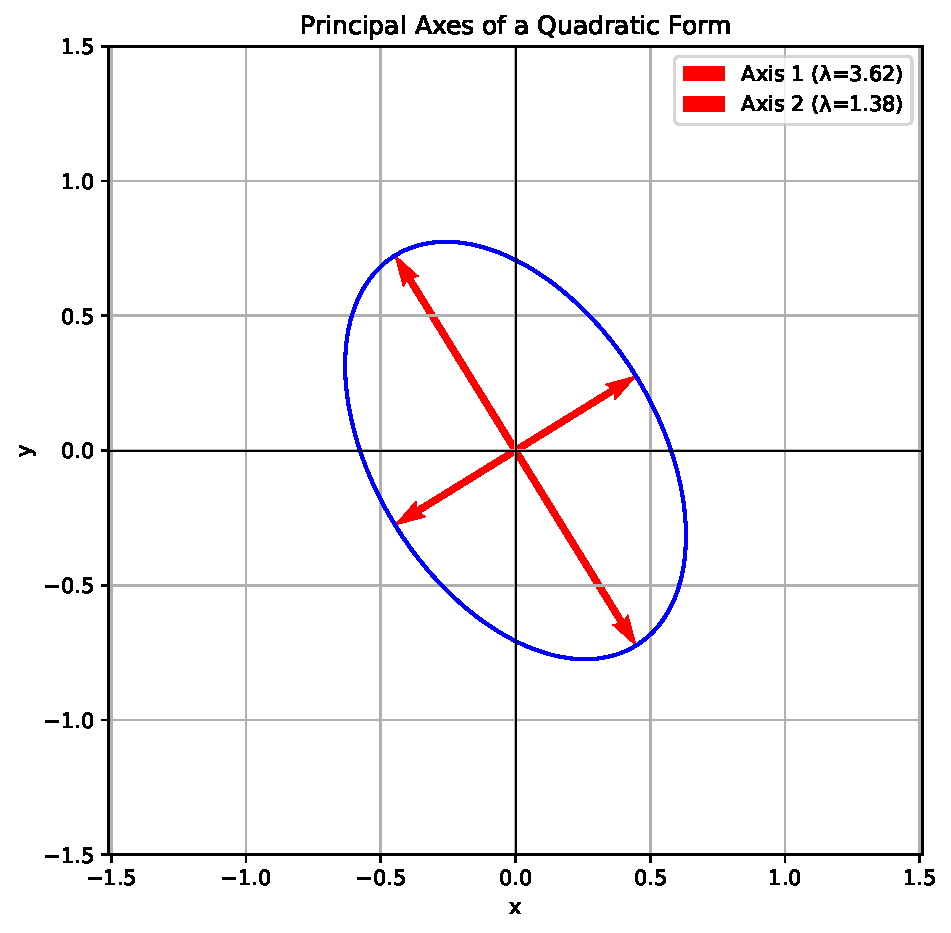
\includegraphics[keepaspectratio]{module2_files/figure-pdf/fig-quadratic-form-output-1.pdf}}

}

\caption{\label{fig-quadratic-form}The ellipse defined by the quadratic
form. The eigenvectors (red) point along the major and minor axes.}

\end{figure}%

The plot shows it perfectly. The quadratic form describes a rotated
ellipse, and the eigenvectors of the associated symmetric matrix point
exactly along its major and minor axes. The signs of the eigenvalues
(\(\lambda_1=5, \lambda_2=-1\)) tell us it's a hyperbola (one positive,
one negative), not an ellipse. My description was slightly off, but the
math and the plot reveal the truth! This is why we do the computation.

\section{Module II Summary}\label{module-ii-summary}

\begin{itemize}
\tightlist
\item
  The core idea of this module is the equation \(Ax = \lambda x\).
\item
  \textbf{Eigenvectors} (\(x\)) are the special directions for a matrix
  that are only scaled, not rotated. \textbf{Eigenvalues} (\(\lambda\))
  are the scaling factors.
\item
  We find eigenvalues by solving the \textbf{characteristic equation}
  \(\det(A - \lambda I) = 0\).
\item
  \textbf{Diagonalization} (\(A = S \Lambda S^{-1}\)) is a powerful tool
  that simplifies matrix powers and reveals the true nature of a
  transformation.
\item
  \textbf{Symmetric matrices} are the nicest of all, with real
  eigenvalues and orthogonal eigenvectors, leading to the decomposition
  \(A = Q \Lambda Q^T\).
\item
  This theory has direct applications in geometry, such as finding the
  principal axes of shapes defined by \textbf{quadratic forms}.
\end{itemize}

\bookmarksetup{startatroot}

\chapter{Module 3: Multivariable Calculus -
Differentiation}\label{module-3-multivariable-calculus---differentiation}

\begin{quote}
\textbf{Syllabus:} Multivariable Calculus - Differentiation Concept of
limit and continuity of functions of two variables - Partial derivatives
of first and higher order - Implicit partial differentiation - Local
linear approximations - Chain rule for derivatives and partial
derivatives - Relative maxima and minima of function of two variables
(finding relative extrema only)
\end{quote}

\begin{longtable}[]{@{}
  >{\raggedright\arraybackslash}p{(\linewidth - 0\tabcolsep) * \real{0.0556}}@{}}
\toprule\noalign{}
\begin{minipage}[b]{\linewidth}\raggedright
\#\# A New Dimension
\end{minipage} \\
\midrule\noalign{}
\endhead
\bottomrule\noalign{}
\endlastfoot
title: ' Module 4- Multi-variable Calculus- Integration' jupyter:
python3 \\
\end{longtable}

\begin{verbatim}



>**Syllabus:** Multivariable Calculus - Integration
Double integrals (Cartesian) - Reversing the order of integration - Change of coordinates (Cartesian to  polar) - Finding areas and volume using double integrals - Mass and centre of gravity of inhomogeneous laminas using double integral - Triple integrals - Volume calculated as triple integral - Triple integral in cylindrical and spherical coordinates (computations involving spheres and cylinders only).

----



`<!-- quarto-file-metadata: eyJyZXNvdXJjZURpciI6Ii4ifQ== -->`{=html}

```{=html}
<!-- quarto-file-metadata: eyJyZXNvdXJjZURpciI6Ii4iLCJib29rSXRlbVR5cGUiOiJjaGFwdGVyIiwiYm9va0l0ZW1OdW1iZXIiOjYsImJvb2tJdGVtRmlsZSI6Im1vZHVsZTUucW1kIiwiYm9va0l0ZW1EZXB0aCI6MH0= -->
```

#  Module 5- Series Representation of Functions 

```````{.quarto-title-block template='C:\Program Files\Quarto\share\projects\book\pandoc\title-block.md'}
---
title: ' Module 5- Series Representation of Functions'

---
\end{verbatim}

\begin{quote}
\textbf{Syllabus:} Series Representation of Functions Taylor series and
Maclaurin series - Binomial series - Fourier series - Euler formulae -
Convergence of Fourier series - Half Range sine and cosine series.
\end{quote}

\begin{center}\rule{0.5\linewidth}{0.5pt}\end{center}

\bookmarksetup{startatroot}

\chapter{Summary}\label{summary}

In summary, this book has no content whatsoever.

\bookmarksetup{startatroot}

\chapter*{References}\label{references}
\addcontentsline{toc}{chapter}{References}

\markboth{References}{References}

\phantomsection\label{refs}




\end{document}
